\documentclass[11pt,letterpaper]{article}
\pdfoutput=1

\usepackage{jheppub}

\usepackage{amsfonts}
\usepackage{amsthm}
\usepackage{bm}
\usepackage{bbm}
\usepackage{mathtools}
\usepackage{booktabs}
\usepackage{tabularx}
\usepackage{threeparttable}
\usepackage{multirow}
\usepackage{float}
\usepackage{enumitem}
\usepackage{adjustbox}
\usepackage{microtype}
\usepackage[T1]{fontenc}
\usepackage[utf8]{inputenc}
\usepackage{xcolor}
\usepackage{tikz}
\usepackage{pgfplots}
\usepackage{etoolbox}
\usetikzlibrary{shapes,arrows,positioning,fit,backgrounds,calc}
\pgfplotsset{compat=1.18}

\hypersetup{
    pdftitle={The Page Curve Is Not Enough: Universality, Ensemble Dependence, and Microscopic Ambiguity in Black Hole Information Recovery},
    pdfauthor={Bernd Johannes Wuebben},
    pdfsubject={Black hole information paradox; Page curve},
    pdfkeywords={Page curve, black hole information paradox, replica wormholes, free probability, Marchenko-Pastur}
}

\newenvironment{figurenotes}{\par\footnotesize\textit{Notes:} }{\par}

\theoremstyle{plain}
\newtheorem{theorem}{Theorem}[section]
\newtheorem{proposition}[theorem]{Proposition}
\newtheorem{lemma}[theorem]{Lemma}
\newtheorem{corollary}[theorem]{Corollary}

\theoremstyle{definition}
\newtheorem{definition}[theorem]{Definition}
\newtheorem{assumption}[theorem]{Assumption}
\newtheorem{example}[theorem]{Example}

\theoremstyle{remark}
\newtheorem{remark}[theorem]{Remark}


\newcommand{\Acal}{\mathcal{A}}
\newcommand{\Bcal}{\mathcal{B}}
\newcommand{\Ccal}{\mathcal{C}}
\newcommand{\Dcal}{\mathcal{D}}
\newcommand{\Ecal}{\mathcal{E}}
\newcommand{\Fcal}{\mathcal{F}}
\newcommand{\Gcal}{\mathcal{G}}
\newcommand{\Hcal}{\mathcal{H}}
\newcommand{\Ical}{\mathcal{I}}
\newcommand{\Jcal}{\mathcal{J}}
\newcommand{\Kcal}{\mathcal{K}}
\newcommand{\Lcal}{\mathcal{L}}
\newcommand{\Mcal}{\mathcal{M}}
\newcommand{\Ncal}{\mathcal{N}}
\newcommand{\Ocal}{\mathcal{O}}
\newcommand{\Pcal}{\mathcal{P}}
\newcommand{\Qcal}{\mathcal{Q}}
\newcommand{\Rcal}{\mathcal{R}}
\newcommand{\Scal}{\mathcal{S}}
\newcommand{\Tcal}{\mathcal{T}}
\newcommand{\Ucal}{\mathcal{U}}
\newcommand{\Vcal}{\mathcal{V}}
\newcommand{\Wcal}{\mathcal{W}}
\newcommand{\Xcal}{\mathcal{X}}
\newcommand{\Ycal}{\mathcal{Y}}
\newcommand{\Zcal}{\mathcal{Z}}

\newcommand{\bzero}{\bm{0}}
\newcommand{\E}{\mathbb{E}}
\newcommand{\Var}{\text{Var}}
\newcommand{\Cov}{\text{Cov}}
\newcommand{\Corr}{\text{Corr}}
\newcommand{\R}{\mathbb{R}}
\newcommand{\N}{\mathbb{N}}
\newcommand{\Z}{\mathbb{Z}}
\newcommand{\C}{\mathbb{C}}
\newcommand{\Prob}{\mathbb{P}}

\newcommand{\F}{\mathcal{F}}
\newcommand{\G}{\mathcal{G}}

\newcommand{\bff}{\bm{f}}
\newcommand{\bh}{\bm{h}}
\newcommand{\bbeta}{\bm{\beta}}
\newcommand{\bSigma}{\bm{\Sigma}}
\newcommand{\bmu}{\bm{\mu}}

\DeclareMathOperator*{\argmin}{arg\,min}
\DeclareMathOperator*{\argmax}{arg\,max}
\DeclareMathOperator{\tr}{tr}
\DeclareMathOperator{\diag}{diag}

\newcommand{\convd}{\xrightarrow{d}}
\newcommand{\convp}{\xrightarrow{p}}
\newcommand{\convas}{\xrightarrow{a.s.}}

\newcommand{\ind}{\mathbbm{1}}
\newcommand{\tavg}[1]{\langle #1 \rangle_t}

\emergencystretch=2em


\preprint{\normalfont\small April 4, 2026 \textperiodcentered{} this version: October 10, 2026}

\title{The Page Curve Is Not Enough:\\
Universality, Ensemble Dependence, and Microscopic Ambiguity in Black Hole
Information Recovery}

\apptocmd{\thebibliography}{\setlength{\itemsep}{3pt plus 0.2ex minus 0.05ex}}{}{\errmessage{Bibliography spacing patch failed}}

\author{Bernd Johannes Wuebben}
\affiliation{New York, NY, USA}
\emailAdd{wuebben@gmail.com}

\abstract{A Page curve constrains radiation entanglement, but its implications for microscopic information recovery depend on which state, ensemble, and channel data are specified. We examine this dependence through explicit finite-dimensional constructions and controlled random-state limits. Two density-matrix ensembles can have the same averaged spectral measure, every averaged replica moment, and the same mean von Neumann entropy, while their entropy and purity fluctuations differ. Fixed Marchenko--Pastur spectra and normalized Wishart spectra give a related large-dimension comparison. At the channel level, an isometry and a replacement channel can reproduce the complete nested radiation trajectory for one input while having different correlations with an external reference. For normalized states, annealed and quenched R\'enyi entropies have the same von Neumann limit; the derivative of their finite-order difference measures the entropy variance. We derive normalized replica-covariance identities and illustrate their normalization with the standard Haar purity covariance, separating these quantities from entropy of an averaged state. Finally, Gaussian and quartic fluctuations with equal variance give different entropy-transition profiles, illustrating the additional role of joint branch fluctuations and reservoir constraints. These calculations delimit what entropy and spectral agreement establish and specify further comparisons needed in gravitational models.}

\keywords{Black hole information paradox, Page curve, replica wormholes, entanglement entropy, universality, Marchenko--Pastur law, free probability, annealed-versus-quenched entropy}

\begin{document}

\notoc
\maketitle

\clearpage
\pagenumbering{roman}
\setcounter{page}{1}
\newpage
\tableofcontents
\newpage
\pagenumbering{arabic}
\setcounter{page}{1}

\emergencystretch=2em


\section{Introduction}
\label{sec01:introduction}

The entropy of Hawking radiation provides a basic test of a proposed
description of black-hole evaporation. Hawking's semiclassical
calculation led to a loss of purity \cite{hawking1976}. For a pure
state evolving unitarily into an accessible final radiation system,
the radiation entropy must eventually return to zero. Page's
random-state calculation provides a quantitative benchmark for the
intermediate entanglement \cite{page1993}. Island and replica-wormhole
calculations have reproduced the expected transition in concrete
gravitational models and connected it to entanglement-wedge
reconstruction \cite{penington2020,almheirietal2019,pssyetal2022}.
The resulting entropy calculations place strong constraints on a
semiclassical description.

The inverse question is different: what properties of the underlying
quantum state, ensemble, or channel are fixed by an entropy curve?
A scalar entropy discards eigenvectors and most eigenvalue information.
An averaged spectral density retains more information, but discards
correlations between eigenvalues in a realization. A trajectory for
one input state does not specify the response to an unknown input or
to an input entangled with a reference. These distinctions matter when
a successful entropy calculation is used to compare microscopic
mechanisms of information recovery.

We study these questions through finite-dimensional constructions and
controlled random-state limits. The purpose is to determine which
inferences require additional data. We do not assume that the principal
approaches to the information problem form mutually exclusive theories,
or that each has a unique radiation spectrum. A comparison between two
gravity models must specify their states, observables, and constraints
before the mathematical examples below can be applied.

\subsection{Explicit comparisons}

The first comparison concerns channels. Given one input and an
isometric evolution, a replacement channel can reproduce the complete
radiation state at every nested release step for that input. The
replacement channel discards unknown input information. A reference
initially maximally entangled with a $D$-dimensional input distinguishes
the final channels: its mutual information with the radiation is
$2\log D$ for the isometry and zero for the replacement. An explicit
sequence of released Bell pairs gives a rising and falling entropy
curve in both cases. This is an elementary channel counterexample,
with no claim that a replacement channel satisfies a gravitational
locality or energy constraint. It states what radiation data from a
single preparation, even when known exactly, can establish on their own.

The second comparison concerns ensembles. We construct two
four-dimensional density-matrix ensembles with the same averaged
spectral measure. Consequently they have the same averaged replica
moments at every positive order and the same mean von Neumann entropy.
One has fluctuating entropy and purity, while the other has a fixed
spectrum and hence no spectral fluctuations. The agreement holds at
finite dimension. A separate comparison between fixed
Marchenko--Pastur quantiles and normalized Wishart matrices shows the
same distinction in the usual large-dimension Page regime. Their
limiting density and entropy correction agree, while their purity
variances differ. These examples isolate the information contained in
one-trace moments from the information in connected two-trace moments.

The third comparison concerns averaging and thermodynamic constraints.
For normalized finite-dimensional density matrices, the annealed and
quenched R\'enyi entropies have the same von Neumann limit. Their
finite-order difference is nonnegative when defined as quenched minus
annealed, and its derivative at order one is half the ensemble variance
of the entropy. We derive this relation and evaluate examples with the
normalization kept inside the ensemble average. We also compare
Gaussian and quartic entropy differences of equal variance: their
averaged-minimum crossover profiles differ. The full profile can
identify the scalar fluctuation law under a fixed-law assumption, but
a marginal heat capacity cannot determine the joint entropy-branch
fluctuations or the associated evaporation dynamics.

\subsection{Relation to established results}

Most of the mathematical ingredients are established. Haar-state
entanglement and its fluctuations provide the finite-dimensional
benchmarks \cite{lubkin1978,page1993,bianchidona2019,giraud2007}.
Unitary designs specify which polynomial averages match Haar measure;
random-circuit results make explicit the dependence on the required
order \cite{brandaoetal2016}. We use a finite-moment statement with its
error dependence, rather than infer an entire entropy trajectory from
a fixed design order. The Marchenko--Pastur law and its non-crossing
moment expansion are standard random-matrix and free-probability
results \cite{nicaspeicher2006}.

On the gravitational side, ref.~\cite{pssyetal2022} supplies a concrete
replica model and also studies reconstruction through the Petz map.
Thus the scope of that work already extends beyond its entropy curve.
The ensemble interpretation of gravitational path integrals has its own
state and factorization questions \cite{saadetal2019,marolfmaxfield2020}.
Bousso and Miyaji explicitly calculate fluctuations of the radiation
entropy in a gravitational model \cite{boussomiyaji2024}. Our normalized
covariance formulas and elementary examples clarify which quantities
such calculations compare; the use of entropy fluctuations as a
probe is not new here.

Energy constraints and fluctuations near competing entropy branches
have likewise been studied in chaotic eigenstates and fixed-area
constructions \cite{murthysrednicki2019,marolfwangwang2020}.
Paper~I derives a broad-distribution correction between an exact planar
spectrum and a level-resolved diagonal approximation in a specified
canonical random-state model \cite{wuebben2026a}. Paper~II studies the
regular, charged-critical, and finite-reservoir fluctuation laws in a
thermodynamic density model \cite{wuebben2026b}. We restate the inputs
needed here and distinguish these two calculations from ensemble
variances of normalized radiation entropies.

The contribution of the present paper is a constructive comparison of
these different inverse questions. The finite examples make their
logical separation explicit, while the random-state and thermodynamic
calculations provide quantitative tests within specified models. The
results do not select a microscopic theory of gravity. They specify
additional comparisons needed before matching entropy curves can be
used to draw that conclusion.

\subsection{Organization and conventions}

Section~\ref{sec02:page_curve_establishes} treats channels and
reference correlations. Section~\ref{sec16:exact_ensembles} gives the
exact finite-dimensional spectral comparison.
Section~\ref{sec03:paper_one_universality}
sets out the random-state moment calculation and the scope of design
matching. Section~\ref{sec04:paper_two_ensemble} treats fluctuating
entropy branches and conserved energy. Design bounds and the comparison at a common spectral limit
are developed in section~\ref{sec05:universality_hierarchy}, and
section~\ref{sec06:annealed_quenched} derives the averaging and
covariance relations. Sections~\ref{sec07:discriminating}
and~\ref{sec08:equilibrium_evaporation} discuss gravitational
comparisons and time-dependent interpretation. The remaining research
questions are collected in section~\ref{sec09:research_program}.
The appendices give the combinatorial, spectral, and probability
calculations used in the text.

All logarithms are natural. Density matrices have unit trace in each
realization unless an unnormalized operator is explicitly introduced.
Averages refer to the ensemble named in the relevant calculation.
A finite-dimensional identity, a large-dimension limit, and a
semiclassical gravity approximation are stated separately. Throughout,
$\gamma=d_R/d_B$ is the radiation-to-black-hole dimension ratio.

\section{What the Page curve establishes}
\label{sec02:page_curve_establishes}

The island calculations recover a turnover of the fine-grained radiation
entropy in controlled semiclassical settings
\citep{penington2020,almheirietal2019,almheirietal2020page,pssyetal2022}.
This is an important constraint on the gravitational description. To state
what follows from the entropy curve alone, however, one must distinguish
the state produced by a specified preparation from the channel that acts
on unknown quantum information. The distinction is standard in quantum
information theory; the examples below make its consequences for a Page
curve explicit. They are finite-dimensional constructions, without a
claim to model local or energy-conserving gravitational dynamics.

\subsection{Entropy of a state and recovery of an input}
\label{subsec02:page_curve_meaning}

Let $A$ be an input system of dimension $D\geq2$. The emitted radiation
after $k$ steps is $R_k=b_1\otimes\cdots\otimes b_k$, and $B_k$ denotes
the remaining system. We use a finite-dimensional tensor factorization;
the identification of the corresponding radiation algebra in gravity is
an additional part of any gravitational application. For a pure state on
$B_kR_k$, the radiation entropy satisfies
\begin{equation}
 S(R_k)=-\tr(\rho_{R_k}\ln\rho_{R_k}),\qquad
 S(R_k)=S(B_k)\leq\min\{\ln d_{R_k},\ln d_{B_k}\}.
 \label{eq02:entropy_bound}
\end{equation}
Approach to this bound is a typicality statement, as in the random-state
calculation of Page~\citep{page1993}. Unitarity alone does not require an
initial rise, a unique maximum, or a particular turnover profile. A
unitary evolution may, for example, emit a product state for a specially
chosen input. A Page-like curve combines the endpoint purity expected
under complete unitary evaporation with assumptions about intermediate
entanglement.

Write $\Ncal_k$ for the completely positive trace-preserving channel from
$A$ to $R_k$. For a specified input $\psi_0=|\psi_0\rangle\langle\psi_0|$,
the entropy data are the numbers $S[\Ncal_k(\psi_0)]$. Information
recovery asks whether the action of $\Ncal_k$ on an input space can be
reversed, including when the input is entangled with a reference. A
single-input entropy curve is therefore a restriction of the data
relevant to recovery. The following elementary construction shows that
even complete knowledge of the radiation density matrices for that
input does not remove this restriction.

\begin{proposition}[Identical radiation histories for one input]
\label{prop02:channel_counterexample}
Let $R_N=b_1\otimes\cdots\otimes b_N$ have dimension at least $D$, and
let $|\Omega\rangle\in R_N$ and $|\psi_0\rangle\in A$ be normalized.
There exist an isometric channel $\Vcal$ and a constant-output channel
$\Ccal$ from $A$ to $R_N$ such that their reductions to every $R_k$
coincide on $\psi_0$. The channel $\Vcal$ has a left inverse on the
input space, whereas $\Ccal$ transmits no information about the input.
\end{proposition}

\begin{proof}
Extend $|\psi_0\rangle$ to an orthonormal basis of $A$, and extend
$|\Omega\rangle$ to an orthonormal set of $D$ vectors in $R_N$. Mapping
the first set to the second defines an isometry $V$ with
$V|\psi_0\rangle=|\Omega\rangle$. Define
\begin{equation}
 \Vcal(X)=VXV^\dagger,\qquad
 \Ccal(X)=\tr(X)\,|\Omega\rangle\langle\Omega|.
 \label{eq02:two_channels}
\end{equation}
Both maps are channels. For every $k$,
\begin{equation}
 \Vcal_k(\psi_0)=\Ccal_k(\psi_0)
 =\tr_{b_{k+1}\cdots b_N}|\Omega\rangle\langle\Omega|,
 \label{eq02:identical_marginals}
\end{equation}
where the subscript denotes restriction of the output to $R_k$.
The map $V^\dagger$ reverses $\Vcal$ on its image and extends to a
trace-preserving recovery channel on all of $R_N$. The output of
$\Ccal$ is independent of its input, so no recovery channel can reverse
it on a space of dimension greater than one.
\end{proof}

These are consistent histories of sequentially released subsystems:
prepare the full output once and emit the factors $b_1,\ldots,b_N$ in
order. Equation~\eqref{eq02:identical_marginals} equates every radiation
observable for the chosen input, including all R\'enyi entropies and
all matrix elements in a specified basis. It does not assert equality for
other inputs. In particular, it establishes a limitation of
single-preparation data rather than an obstruction to quantum channel
tomography.

\subsection{An exact rising and falling entropy curve}
\label{subsec02:bell_example}

An explicit choice of the output illustrates the proposition. Take
$N=2q$ qubits and pair qubit $j$ with qubit $q+j$:
\begin{equation}
 |\Omega\rangle
 =\bigotimes_{j=1}^{q}
 \frac{|0\rangle_j|0\rangle_{q+j}
       +|1\rangle_j|1\rangle_{q+j}}{\sqrt2}.
 \label{eq02:bell_output}
\end{equation}
For $k\leq q$, every emitted qubit is one half of a Bell pair whose
other half remains inside, so $\rho_{R_k}$ is maximally mixed. For
$k>q$, each additional emission completes one of those pairs. The
number of pairs crossing the radiation cut is therefore
$\min(k,2q-k)$, giving exactly
\begin{equation}
 S(R_k)=\min(k,2q-k)\ln2,\qquad 0\leq k\leq2q.
 \label{eq02:bell_curve}
\end{equation}
For six qubits, the entropies in units of $\ln2$ are
$0,1,2,3,2,1,0$. The final radiation state is pure. The proposition
produces this same trajectory under an information-preserving channel
and an input-erasing channel. The example is deliberately simple: its
linear branches and flat nonzero entanglement spectrum are not the
finite-size Haar profile. Any desired pure multipartite output,
including a Haar-typical one, can instead be used in the proposition.

The constant-output channel is often called a \emph{replacer channel}.
It has a globally isometric realization
\begin{equation}
 W|\psi\rangle_A
 =|\Omega\rangle_{R_N}\otimes|\psi\rangle_E,
 \qquad \Ccal(X)=\tr_E(WXW^\dagger),
 \label{eq02:replacer_dilation}
\end{equation}
where $E$ is an unobserved system of dimension $D$. The input has moved
to $E$; it has not been destroyed by the enlarged evolution. Thus the
example does not contradict unitarity of a closed system. It shows
that purity of the observed radiation does not certify that the
radiation contains the input. If one independently assumes that the
complete evolution is an isometry and that no complementary output
remains, recovery follows from those assumptions. They are not implied
by the curve. Equation~\eqref{eq02:replacer_dilation} also identifies
why this construction is not a model of complete black-hole
evaporation with a proven absence of remnants or hidden sectors.

\subsection{An external reference distinguishes the channels}
\label{subsec02:reference_test}

The relevant distinction can be measured by entangling the input with
a reference, as in quantum communication and the Hayden--Preskill
recovery problem~\citep{schumacher1996,haydenpreskill2007}. Let
\begin{equation}
 |\Phi_D\rangle_{QA}=\frac1{\sqrt D}
 \sum_{i=1}^{D}|i\rangle_Q|i\rangle_A,
 \qquad |\Psi_V\rangle=(I_Q\otimes V)|\Phi_D\rangle.
 \label{eq02:reference_input}
\end{equation}
The two final joint states are
\begin{equation}
 \rho_{QR_N}^{\Vcal}=|\Psi_V\rangle\langle\Psi_V|,
 \qquad
 \rho_{QR_N}^{\Ccal}=\frac{I_Q}{D}\otimes
 |\Omega\rangle\langle\Omega|.
 \label{eq02:reference_outputs}
\end{equation}
Consequently their mutual information, defined by
$I(Q:R)=S(Q)+S(R)-S(QR)$, is
\begin{equation}
 I(Q:R_N)_{\Vcal}=2\ln D,
 \qquad I(Q:R_N)_{\Ccal}=0.
 \label{eq02:reference_mutual_information}
\end{equation}
This is a different input preparation from the pure-state experiment
in equation~\eqref{eq02:identical_marginals}. For the reference-entangled
input, an information-preserving channel produces mixed radiation
entangled with $Q$; requiring its radiation entropy to vanish would
be the wrong recovery criterion.

One can also compare with the ideal encoded state through
\begin{equation}
 F_V(\Ncal)=\langle\Psi_V|
 (\operatorname{id}_Q\otimes\Ncal)
 (|\Phi_D\rangle\langle\Phi_D|)|\Psi_V\rangle.
 \label{eq02:encoding_fidelity}
\end{equation}
For the two channels,
\begin{equation}
 F_V(\Vcal)=1,
 \qquad F_V(\Ccal)=\frac1{D^2}.
 \label{eq02:reference_fidelities}
\end{equation}
Indeed, substituting the second state in
equation~\eqref{eq02:reference_outputs} gives
$D^{-2}\sum_i|\langle\Omega|V|i\rangle|^2=D^{-2}$, because
$|\Omega\rangle$ lies in the image of $V$. Applying a decoder that
inverts $V$ on this image gives the usual entanglement fidelity for
the maximally mixed input~\citep{schumacher1996}. Every decoder applied
to a replacer still produces a constant-output channel, whose
entanglement fidelity for that input is $D^{-2}$. These comparisons
distinguish transmission of quantum information from purification of a
specified output state without requiring a reconstruction of every
matrix element of the channel.

Full reference-assisted state tomography supplies a stronger positive
result. For the maximally entangled input above, define the normalized
Choi state of a channel $\Ncal:A\to R$ by
\begin{equation}
 J_{\Ncal}=(\operatorname{id}_Q\otimes\Ncal)
 (|\Phi_D\rangle\langle\Phi_D|)
 =\frac1D\sum_{i,j}|i\rangle\langle j|_Q
       \otimes\Ncal(|i\rangle\langle j|).
 \label{eq02:choi_state}
\end{equation}
The entire state $J_{\Ncal}$ determines the channel on every input:
\begin{equation}
 \Ncal(\omega)=D\,\mathrm{Tr}_Q
       [(\omega^{\mathsf T}\otimes I_R)J_{\Ncal}],
 \label{eq02:choi_inversion}
\end{equation}
where the transpose is taken in the basis defining $|\Phi_D\rangle$.
This is the standard channel-state correspondence \cite{choi1975}; the
formula follows by contracting the displayed matrix units. Thus one
suitably entangled preparation with complete joint-state information
can determine a channel. Entropy or selected reference correlators
retain only part of that information. The single-input counterexample
concerns a fixed unentangled input, and does not apply to tomography of
$J_{\Ncal}$.

\subsection{Spectral information and preparation averages}
\label{subsec02:spectral_limitations}

Even at a fixed time, the complete entanglement spectrum does not
determine the density matrix relative to specified physical
observables. For example, let
\begin{equation}
 \rho=\begin{pmatrix}p&0\\0&1-p\end{pmatrix},\qquad
 H=\frac1{\sqrt2}\begin{pmatrix}1&1\\1&-1\end{pmatrix},\qquad
 \rho'=H\rho H^\dagger,
 \label{eq02:isospectral_states}
\end{equation}
with $0<p<1$ and $p\ne1/2$. These states have identical R\'enyi
entropies at every order. Holding the observable
$Z=\diag(1,-1)$ fixed, however,
\begin{equation}
 \tr(\rho Z)=2p-1,
 \qquad \tr(\rho' Z)=0.
 \label{eq02:isospectral_observable}
\end{equation}
The comparison concerns different states in the same physical basis,
not a simultaneous relabeling of states and observables. Spectral
statistics can distinguish some state ensembles, but they do not
specify the eigenvectors, an encoding map, or the dynamics that
produced the states. Proposition~\ref{prop02:channel_counterexample}
gives the stronger statement that even full state information for a
fixed unentangled input cannot determine the channel on other inputs.

A separate distinction concerns averaging. In matrix-integral
descriptions of JT gravity, the gravitational observables have an
ensemble interpretation~\citep{saadetal2019,marolfmaxfield2020}.
Other averages can refer to states or circuits within a fixed theory.
These operations should be specified independently of whether the
underlying Hamiltonian is fixed. For normalized density matrices in
a common finite-dimensional space, differentiation at replica number
one gives exactly
\begin{equation}
 -\left.\partial_n\ln\E\tr\rho^n\right|_{n=1}
 =\E[-\tr(\rho\ln\rho)].
 \label{eq02:replica_derivative}
\end{equation}
The equality follows from $\tr\rho=1$ and differentiation under the
average; $x\ln x$ is bounded on $[0,1]$. The entropy of the averaged
state, $S(\E\rho)$, is a different observable. Approximating replica
moments or taking a dimension limit before the derivative can require
additional control, but it does not change this exact
finite-dimensional identity. Section~\ref{sec06:annealed_quenched}
treats the finite-order R\'enyi distinction and entropy fluctuations.

The scope of the argument is consequently precise. A Page curve tests
a property of radiation states in a specified preparation. Additional
spectral information tests further properties of those states and of
their distribution. Recovery tests how the radiation depends on an
input, including its entanglement with a reference. The examples in
this section separate these questions; they do not assert that two
fully specified gravitational theories agree on every such test.

\section{Identical averaged spectra and distinct fluctuations}
\label{sec16:exact_ensembles}
\label{subsec05:exact_spectral_example}

An averaged spectral measure contains the expectation of every linear
spectral statistic, including the von Neumann entropy.  It need not
determine the covariance of two such statistics.  The following
four-dimensional example demonstrates this distinction exactly, without
a limiting argument.  It is an explicit application of the standard
difference between one-point and two-point probability data.

Set $c=1/4$ and choose $0\leq u<v<c$.  Define three normalized spectra,
\begin{equation}
\label{eq05:exact_spectra}
 \begin{aligned}
 L_u&=(c+u,c-u,c+u,c-u),\\
 L_v&=(c+v,c-v,c+v,c-v),\\
 L_{uv}&=(c+u,c-u,c+v,c-v).
 \end{aligned}
\end{equation}
Ensemble $\mathcal A$ chooses $L_u$ or $L_v$ with equal probabilities;
ensemble $\mathcal B$ always uses $L_{uv}$.  In each case conjugate the
diagonal state by an independent Haar unitary in $U(4)$.  All states
are full rank and can be purified with an environment of dimension at
least four.  Each ensemble has averaged density matrix $I_4/4$.

\begin{proposition}[Exact matching of averaged spectral data]
\label{prop05:exact_spectral_separation}
The ensembles $\mathcal A$ and $\mathcal B$ have identical averaged
spectral measures.  In particular, for every function $g$ defined on
the four eigenvalue values,
\begin{equation}
\label{eq05:exact_linear_matching}
 \mathbb E_{\mathcal A}\mathrm{Tr}\,g(\rho)
 =\mathbb E_{\mathcal B}\mathrm{Tr}\,g(\rho).
\end{equation}
They therefore have identical $\mathbb E\mathrm{Tr}\rho^n$ for all
real $n>0$ and identical mean von Neumann entropy.  Nonetheless,
\begin{align}
\label{eq05:exact_purity_variance}
 \mathrm{Var}_{\mathcal A}(\mathrm{Tr}\rho^2)
 &=4(u^2-v^2)^2>0,
 &\mathrm{Var}_{\mathcal B}(\mathrm{Tr}\rho^2)&=0,\\
\label{eq05:exact_entropy_variance}
 \mathrm{Var}_{\mathcal A}S(\rho)
 &=[f(u)-f(v)]^2>0,
 &\mathrm{Var}_{\mathcal B}S(\rho)&=0,
\end{align}
where $f(t)=-(c+t)\log(c+t)-(c-t)\log(c-t)$.
\end{proposition}

\begin{proof}
Each of $c+u,c-u,c+v,c-v$ occurs once in the average of the counting
measures of $L_u$ and $L_v$, and once in the counting measure of
$L_{uv}$.  This proves Eq.~\eqref{eq05:exact_linear_matching}.
The purity in ensemble $\mathcal A$ takes the values $1/4+4u^2$
and $1/4+4v^2$, whereas it is constant in $\mathcal B$.
The variance of two equally probable numbers is one quarter of their
squared difference, giving Eq.~\eqref{eq05:exact_purity_variance}.
The corresponding entropies are $2f(u)$ and $2f(v)$ in $\mathcal A$
and $f(u)+f(v)$ in $\mathcal B$.  Finally,
$f'(t)=\log[(c-t)/(c+t)]<0$ for $0<t<c$, so the entropy variance
in $\mathcal A$ is strictly positive.
\end{proof}

For example, $u=0$ and $v=1/8$ give the common mean purity $9/32$
and common mean entropy
\begin{equation}
\label{eq05:exact_example_values}
 \mathbb E S=\frac52\log2-\frac38\log3,
 \qquad
 \mathrm{Var}_{\mathcal A}(\mathrm{Tr}\rho^2)=\frac1{1024},
 \qquad
 \mathrm{Var}_{\mathcal A}S
 =\frac14\left(\frac34\log3-\log2\right)^2.
\end{equation}
Both variances vanish in $\mathcal B$.  Since the averaged density
matrix and mean entropy also agree, the quantity
$S(\mathbb E\rho)-\mathbb E S(\rho)$ is identical in these two
ensembles.  That concavity gap therefore does not determine the
entropy variance either.

This comparison is stronger than matching finitely many moments or a
limiting density: it matches all averaged one-point spectral data at
finite dimension.  An exact mean von Neumann entropy and every averaged
replica trace still leave fluctuation data undetermined.  Products of
traces, rather than additional single-trace orders alone, detect the
difference.  In particular, the annealed R\'enyi entropies agree in
these ensembles, while their averaged R\'enyi entropies can differ
because the logarithm is applied before averaging.  The distinction
and its relation to Eq.~\eqref{eq05:exact_entropy_variance} are made
precise in Section~\ref{sec06:annealed_quenched}.


\section{The normalized random-state benchmark}
\label{sec03:paper_one_universality}

A useful comparison between microscopic models requires a precisely
specified reference ensemble.  We use the reduced state of a complex
Haar-random pure state.  Its finite-dimensional moments, limiting
Marchenko--Pastur law, and entropy are standard results
\cite{lubkin1978,lloydpagels1988,page1993,sen1996,nicaspeicher2006}.
They also describe the equal-weight, fixed-dimension limit of the
replica model studied by Penington et al.~\cite{pssyetal2022}.
The role of this benchmark is to identify which spectral data coincide
under specified assumptions.  It does not assert that every gravitational
replica calculation belongs to the same random-matrix ensemble.

\subsection{Exact normalization and finite-dimensional moments}
\label{subsec03:non_crossing_sum}

Let $\mathcal H_R=\mathbb C^m$ and $\mathcal H_B=\mathbb C^b$, with
$m=d_R$, $b=d_B$, and $\gamma=m/b$.  For a normalized Haar-random vector
$|\psi\rangle\in\mathcal H_R\otimes\mathcal H_B$, set
$\rho_R=\mathrm{Tr}_B|\psi\rangle\langle\psi|$.  Equivalently, if
$G$ is an $m\times b$ matrix of independent standard complex Gaussian
entries, then
\begin{equation}
\label{eq03:normalized_wishart}
 \rho_R=\frac{GG^\dagger}{\mathrm{Tr}(GG^\dagger)}.
\end{equation}
Normalization is imposed for each realization.  Replacing the denominator
by its expectation gives a different finite-dimensional random matrix.
Although this replacement preserves the limiting density, it need not
preserve the leading coefficient of a connected fluctuation.

Write $c(\pi)$ for the number of cycles of a permutation, let
$\tau_k=(1\,2\cdots k)$, and define the rising factorial
$(D)_k=D(D+1)\cdots(D+k-1)$ with $D=mb$.  The exact moment is
\begin{equation}
\label{eq03:haar_moment}
 \mathbb E_{\mathrm H}\,\mathrm{Tr}\rho_R^k
 =\frac{1}{(mb)_k}
  \sum_{\pi\in S_k}b^{c(\pi)}m^{c(\tau_k\pi)}.
\end{equation}
Appendix~\ref{sec12:appendix_paper_one} derives this expression from the
symmetric projector and gives the corresponding formula for products of
traces.  In particular,
\begin{equation}
\label{eq03:exact_purity}
 \mathbb E_{\mathrm H}\,\mathrm{Tr}\rho_R=1,
 \qquad
 \mathbb E_{\mathrm H}\,\mathrm{Tr}\rho_R^2
 =\frac{m+b}{mb+1}.
\end{equation}
The second identity is Lubkin's mean-purity formula~\cite{lubkin1978}.
Both identities hold at arbitrary positive integer dimensions, including
$m=1$ or $b=1$.  They provide simple normalization checks before any
large-dimension expansion is made.

For fixed $k$ and $m,b\to\infty$ with $m/b\to\gamma\in(0,\infty)$,
Eq.~\eqref{eq03:haar_moment} becomes
\begin{equation}
\label{eq03:narayana_moment}
 m^{k-1}\mathbb E_{\mathrm H}\,\mathrm{Tr}\rho_R^k
 \longrightarrow M_k(\gamma)
 =\sum_{j=1}^k\frac1k\binom{k}{j}\binom{k}{j-1}\gamma^{k-j}.
\end{equation}
The power multiplying the physical moment is $m^{k-1}$, because the
spectral measure below describes $m\lambda$, where $\lambda$ is an
eigenvalue of $\rho_R$.  Thus $M_2=1+\gamma$ corresponds to the physical
purity $m^{-1}+b^{-1}$ at leading order.  The finite-dimensional formula
and its limiting form should be distinguished throughout.

The leading terms in the permutation sum satisfy
$c(\pi)+c(\tau_k\pi)=k+1$ and are indexed by non-crossing partitions.
Their Narayana multiplicities give Eq.~\eqref{eq03:narayana_moment}.
Keeping only the identity and the inverse full cycle, for $k\geq2$,
would instead give
\begin{equation}
\label{eq03:two_saddle}
 \bigl(\mathbb E\,\mathrm{Tr}\rho_R^k\bigr)_{\mathrm{two\ terms}}
 \sim m^{1-k}+b^{1-k}
 =m^{1-k}(1+\gamma^{k-1}).
\end{equation}
At $\gamma=1$, the full limiting moment is the Catalan number
$C_k=(k+1)^{-1}\binom{2k}{k}$.  The ratio of the complete leading sum
to the two retained terms is $C_k/2$, equal to $1,5/2,7$ for
$k=2,3,4$.  Consequently, the two terms reproduce purity at leading
order but miss the higher-moment transition even within this benchmark.
These are standard non-crossing-partition facts concerning the stated
random-state benchmark.

\subsection{The limiting density and entropy}
\label{subsec03:marchenko_pastur}

For eigenvalues $\lambda_i$ of $\rho_R$, define the empirical probability
measure $\nu_m=m^{-1}\sum_{i=1}^m\delta_{m\lambda_i}$.  Its limiting
Marchenko--Pastur measure is
\begin{equation}
\label{eq03:mp_density}
 d\mu_\gamma(x)=
 \frac{\sqrt{(x_+-x)(x-x_-)}}{2\pi\gamma x}
 \mathbf1_{[x_-,x_+]}(x)\,dx
 +(1-\gamma^{-1})_+\delta_0(dx),
 \qquad x_\pm=(1\pm\sqrt\gamma)^2.
\end{equation}
It has total mass one and first moment one.  The atom for $\gamma>1$
accounts for the $m-b$ zero eigenvalues of a rank-$b$ radiation state.
The density is a law for the \emph{scaled} eigenvalues $x$, rather than
for the eigenvalues $\lambda$ themselves.

The entropy can be expressed without an analytic continuation of an
integer-index polynomial:
\begin{equation}
\label{eq03:entropy_density}
 S(\rho_R)=\log m-\int x\log x\,d\nu_m(x),
 \qquad 0\log0:=0.
\end{equation}
For $0<\gamma\leq1$, the integral against $\mu_\gamma$ is $\gamma/2$.
The exact mean entropy, conjectured by Page and subsequently proved
\cite{page1993,sen1996}, is
\begin{equation}
\label{eq03:page_formula}
 \mathbb E_{\mathrm H}S(\rho_R)
 =H_{mb}-H_b-\frac{m-1}{2b}
 =\log m-\frac{\gamma}{2}+o(1),
 \qquad m\leq b,
\end{equation}
where $H_j=\sum_{r=1}^j r^{-1}$.  For $m>b$, exchange $m$ and $b$,
since the two reduced states of a pure bipartite state have the same
nonzero spectrum.  In terms of the dimension detuning
$\delta=\log b-\log m$, the leading expression on either side is
\begin{equation}
\label{eq03:page_correction}
 \mathbb E_{\mathrm H}S(\rho_R)
 =\min(\log m,\log b)-\tfrac12e^{-|\delta|}+o(1).
\end{equation}
Here $\delta$ parametrizes a family of bipartite ensembles.  A physical
time-dependent Page curve additionally requires a rule for the evolution
of the subsystem dimensions and states; Eq.~\eqref{eq03:page_correction}
alone does not provide that rule.

\subsection{Which ingredients are universal?}
\label{subsec03:free_probability}

The free moment--cumulant relation is
\begin{equation}
\label{eq03:free_cumulants}
 M_k=\sum_{\pi\in NC(k)}\prod_{V\in\pi}r_{|V|}.
\end{equation}
For the measure in Eq.~\eqref{eq03:mp_density}, $r_j=\gamma^{j-1}$
and hence $R(z)=\sum_{j\geq1}r_jz^{j-1}=(1-\gamma z)^{-1}$
\cite{speicher1994,nicaspeicher2006}.  The two inputs are the
non-crossing combinatorics and the particular cumulant weights.
Planarity by itself fixes neither those weights nor freeness of an
arbitrary family of operators.  For example, a semicircular variable
has only its second free cumulant nonzero and has a different planar
moment sequence.  Energy-dependent weights and constraints in a
radiation model likewise require their own spectral calculation.

The relevant lesson of Paper~I~\cite{wuebben2026a} is therefore
conditional: in the equal-weight fixed-dimension limit, the complete
planar calculation has the same leading spectral data as this normalized
random-state benchmark.  The thermally weighted planar spectrum treated
there requires further input; it cannot in general be replaced by a
Gaussian average of the fixed-dimension entropy at order one.
Section~\ref{sec04:paper_two_ensemble} treats the thermodynamic assumptions
separately.  Neither a genus expansion nor a matching mean heat capacity
alone identifies the complete radiation ensemble.

\subsection{What a matching density establishes}
\label{subsec03:consequence}

A limiting density determines its integrable one-point spectral
statistics.  It does not determine the joint distribution of eigenvalues,
their finite-dimensional covariance, the eigenvectors, or correlations
with an external reference.  In particular, two ensembles may have the
same limiting moments and entropy while assigning different probabilities
to deviations from those values.  Section~\ref{sec05:universality_hierarchy}
constructs such a pair explicitly, using the density in
Eq.~\eqref{eq03:mp_density}.  This makes the limitation of the Page
benchmark a statement about specified mathematical objects, without
assuming that a named microscopic proposal realizes either ensemble.

\section{Thermodynamic fluctuations and the observable being averaged}
\label{sec04:paper_two_ensemble}

A Page transition involves a comparison of entropies. The distribution of
that comparison depends on both the preparation and the observable. A
heat capacity supplies useful information about energy fluctuations in a
specified equilibrium ensemble, but does not specify an arbitrary
entanglement-entropy crossover. This section separates these ingredients
and explains the role of the results of Papers~I and~II
\cite{wuebben2026a,wuebben2026b}. All entropies are dimensionless, with
Boltzmann's constant set to one.

\subsection{Averaging two competing branches}

Let $F_1$ and $F_2$ be integrable random entropy branches. Write
$F_i=\overline F_i+\eta_i$, where $\E\eta_i=0$, and define
\begin{equation}
 \Delta=\overline F_1-\overline F_2,\qquad
 \xi=\eta_1-\eta_2.
 \label{eq04:branch_difference}
\end{equation}
The exact algebraic identity
\begin{equation}
 \E\min(F_1,F_2)=\overline F_2+\E\min(\Delta+\xi,0)
 \label{eq04:averaged_minimum}
\end{equation}
does not require independence between the branches. In a model in which
an entropy is approximated by the minimum of two branches, it specifies
the correction caused by fluctuations. The identification of those
branches with generalized entropies in gravity requires a separate
state and replica calculation; it is not part of the algebraic identity.
Fixed-area and chaotic-eigenstate treatments provide concrete settings
for such calculations \cite{marolfwangwang2020,murthysrednicki2019}.

The deficit relative to the minimum of the means is
\begin{equation}
 B_\xi(\Delta)
 =\min(\Delta,0)-\E\min(\Delta+\xi,0)
 =\frac{\E|\Delta+\xi|-|\Delta|}{2}\geq0.
 \label{eq04:deficit}
\end{equation}
The last inequality follows from convexity of the absolute value. At
the crossing, $B_\xi(0)=\E|\xi|/2$. In particular, the width measured by
$\sqrt{\Var\xi}$ and the central deficit measure different features of
the law. For a Gaussian difference of standard deviation $\sigma$,
\begin{equation}
 B_{\mathrm G}(\Delta)
 =\sigma\phi(\Delta/\sigma)
   -|\Delta|\Phi(-|\Delta|/\sigma),
 \qquad B_{\mathrm G}(0)=\frac{\sigma}{\sqrt{2\pi}},
 \label{eq04:gaussian}
\end{equation}
where $\phi$ and $\Phi$ are the standard normal density and distribution
function. The zero-width limit is taken separately and gives $B=0$.

There is also a positive identification result within this model. Hold
the law of $\xi$ fixed while varying $\Delta$ and put
$h(\Delta)=\E\min(\Delta+\xi,0)$. If $\xi$ has density $f_\xi$, then
\begin{equation}
 h'(\Delta)=\Prob(\xi<-\Delta),\qquad
 h''(\Delta)=-f_\xi(-\Delta).
 \label{eq04:inverse_profile}
\end{equation}
The first equality follows by differentiating a Lipschitz integrand;
the second follows wherever the density is continuous. With atoms,
one-sided derivatives give the corresponding distribution function.
Thus an exact crossover as a function of a calibrated entropy difference
can determine this one-dimensional fluctuation law. This observation
also specifies the limits of the inference: it identifies neither the
joint law of $F_1,F_2$ nor the channel that prepares them. If the law
changes with $\Delta$, its variation contributes to the derivative, and
\eqref{eq04:inverse_profile} is no longer an inversion formula for a
single distribution.

\subsection{Equal widths and different crossover shapes}

Consider a standard normal variable $Y_{\mathrm G}$ and the unit-variance
quartic variable $Y_{\mathrm Q}=X/\sqrt v$, where
\begin{equation}
 p_X(x)=\frac{2}{\Gamma(1/4)}e^{-x^4},\qquad
 v=\frac{\Gamma(3/4)}{\Gamma(1/4)}.
 \label{eq04:quartic}
\end{equation}
Both variables have mean zero and variance one. Their central deficits
are nevertheless different:
\begin{equation}
 B_{Y_{\mathrm G}}(0)=\frac{1}{\sqrt{2\pi}}
 \simeq0.398942,\qquad
 B_{Y_{\mathrm Q}}(0)=2^{-5/4}\simeq0.420448.
 \label{eq04:equal_variance}
\end{equation}
The quartic value follows from the gamma-function moments in
appendix~\ref{sec13:appendix_paper_two}. Their curvature profiles also
differ, because they reproduce different densities in
\eqref{eq04:inverse_profile}. Figure~\ref{fig04:equal_variance} compares
the two complete functions without fitting either shape.

\begin{figure}[tbp]
 \centering
 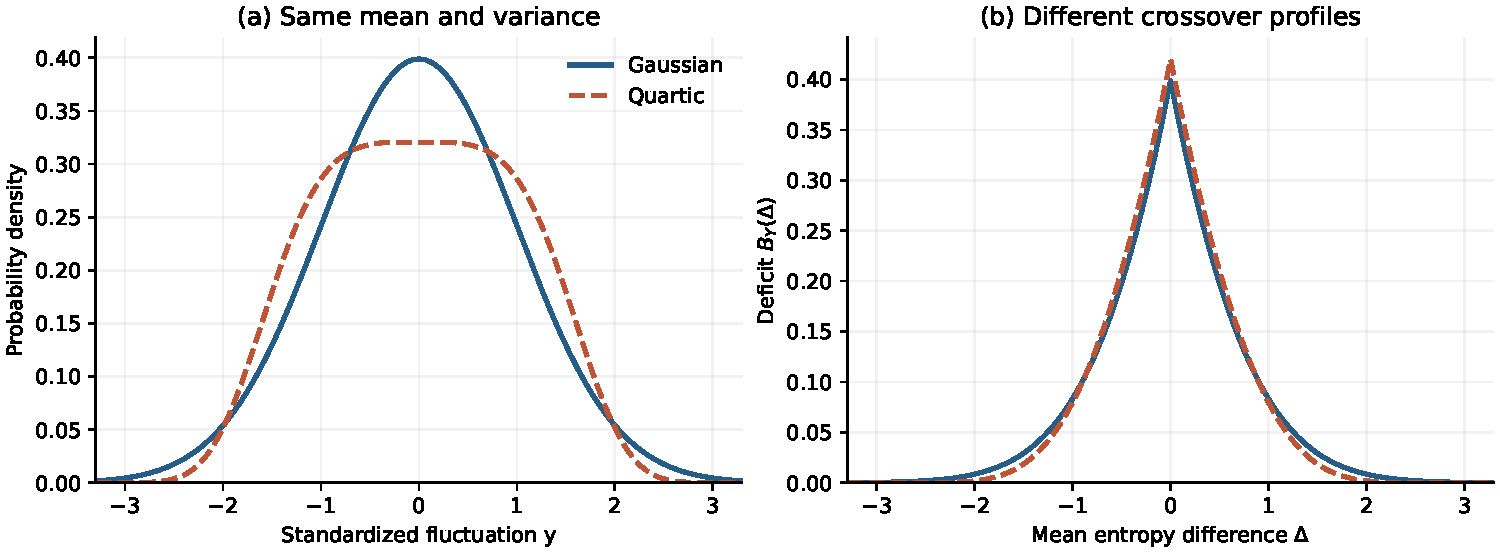
\includegraphics[width=\textwidth]{figures/output/fig04_equal_variance.pdf}
 \caption{Equal variance does not determine the averaged-minimum
 crossover. Left: standard normal and standardized quartic densities,
 each with mean zero and variance one. Right: their deficits
 $B_Y(\Delta)$ from \eqref{eq04:deficit}, evaluated by deterministic
 quadrature. The central values are given in
 \eqref{eq04:equal_variance}. These are probability models for a
 fluctuating entropy difference; no evaporation trajectory is assumed.}
 \label{fig04:equal_variance}
\end{figure}

Even the variance of a branch difference requires joint information:
\begin{equation}
 \Var\xi=\Var\eta_1+\Var\eta_2-2\Cov(\eta_1,\eta_2).
 \label{eq04:covariance}
\end{equation}
For two centered Gaussian branches, each with variance $s^2$ and
correlation $c$, this gives $\Var\xi=2s^2(1-c)$. With the same marginal
branch laws, the crossover width therefore ranges from zero at $c=1$
to $2s$ at $c=-1$. These endpoints describe degenerate but well-defined
joint Gaussian laws. A common fluctuating contribution cancels from the
difference, whereas an anticorrelated contribution is amplified.

\subsection{Regular phases, finite reservoirs, and criticality}

For a temperature-independent density of states, the exact canonical
identity is $\Var E=T^2 C_{\rm can}$, where
$C_{\rm can}=\partial_T\E E$. At a stable, sharply concentrated saddle,
$C_{\rm can}$ agrees to leading order with the saddle heat capacity
$C_B>0$. Linearizing a thermodynamic entropy using
$\mathrm d S_B/\mathrm d E=1/T$ then gives $\Var S_B\simeq C_B$ when
higher-order fluctuations are negligible. This concerns the fluctuating
thermodynamic function $S_B(E)$. The capacity of entanglement of a
normalized state is instead
\begin{equation}
 C_{\mathrm{ent}}(\rho)
 =\mathrm{Tr}\rho(\log\rho)^2
   -\bigl(\mathrm{Tr}\rho\log\rho\bigr)^2.
 \label{eq04:entanglement_capacity}
\end{equation}
For a Gibbs state it equals $\beta^2\Var E$; for a general radiation
state it need not equal a black-hole heat capacity. It also differs
from the ensemble variance of $S(\rho)$ studied in
section~\ref{sec06:annealed_quenched}.

Fixing the energy of a composite system permits exchange between its
subsystems. In a density-of-states approximation,
\begin{equation}
 p(E_B)\propto
 \exp\{S_B(E_B)+S_R(E_{\rm tot}-E_B)\}.
 \label{eq04:finite_bath}
\end{equation}
At a common-temperature stationary point, the Gaussian variance is
$T^2 C_{\rm eff}$, with
\begin{equation}
 C_{\rm eff}=(C_B^{-1}+C_R^{-1})^{-1},\qquad
 C_B^{-1}+C_R^{-1}>0.
 \label{eq04:effective_capacity}
\end{equation}
The inequality is the local stability condition. The linear entropy
variations are $\delta S_B=\delta E_B/T$ and
$\delta S_R=-\delta E_B/T$, so that
$\Var(S_B-S_R)\simeq4C_{\rm eff}$.
These relations underlie enhanced entanglement corrections in
energy-constrained chaotic systems \cite{murthysrednicki2019}.
For a negative $C_B$ and positive $C_R$, local stability is possible if
$C_R<|C_B|$. Global phase dominance and an actual physical confinement
mechanism are additional questions. Fixing $E_B$ itself removes this
classical exchange fluctuation; fixing $E_{\rm tot}$ does not.

Paper~II gives a non-Gaussian example in its specified RN--AdS
thermodynamic density model \cite{wuebben2026b}. In $d+1\geq4$ bulk
dimensions at the charged critical point, set $N=S_c$ and
\begin{equation}
 a_d=\frac{(d-1)(2d-3)}{24},\qquad
 L_N=(d-1)a_d^{-1/4}N^{3/4}.
 \label{eq04:critical_scale}
\end{equation}
The centered black-hole entropy divided by $L_N$ tends to the quartic
law in \eqref{eq04:quartic}. A regular finite reservoir changes this to
\begin{equation}
 p_u(x)=Z_u^{-1}e^{-x^4-ux^2},\qquad
 u=\lim_{N\to\infty}\frac{L_N^2}{2C_R}.
 \label{eq04:critical_bath}
\end{equation}
The result assumes the local reservoir expansion and the tail and
moment control stated in appendix~\ref{sec13:appendix_paper_two}.
A reservoir of capacity much larger than $N^{3/2}$ retains the canonical
quartic law. Capacities of order $N^{3/2}$ change its shape. A diverging
but smaller regular reservoir produces a Gaussian law on its own
narrower scale. These are different preparations of the same critical
black-hole family.

To transfer such a law to generalized entropies $F_{1,N},F_{2,N}$, one
must also control their response to the critical mode. For example, if
\begin{equation}
 \frac{(F_{1,N}-F_{2,N})-\E(F_{1,N}-F_{2,N})}{L_N}
 =aX_N+r_N,\qquad \E r_N^2\longrightarrow0,
 \label{eq04:response}
\end{equation}
with $X_N$ converging in distribution and second moment to $p_u$, then
the limiting variance is $a^2\Var_{p_u}X$ and the averaged-minimum
profile follows from the law of $aX$. This is a conditional transfer
statement. If $a=0$, this mode contributes no leading width on the
$L_N$ scale. A thermodynamic critical point alone does not determine $a$.

The charged critical point must also be distinguished from a first-order
transition and a metastable spinodal. At the neutral AdS temperature
minimum, the Gaussian saddle expansion fails as two black-hole branches
meet. The Hawking--Page transition instead compares the free energies
of thermal AdS and a black hole \cite{hawkingpage1983}. These events
occur at different radii and support different fluctuation analyses.

\subsection{Averaging sector entropies and combining spectra}

There is a further distinction between a classical mixture of entropy
values and the spectrum of the resulting quantum state. If radiation
resolves mutually orthogonal sectors,
\begin{equation}
 \rho_R=\bigoplus_\alpha p_\alpha\rho_{R,\alpha},\qquad
 S(\rho_R)=H(p)+\sum_\alpha p_\alpha S(\rho_{R,\alpha}),
 \label{eq04:sector_entropy}
\end{equation}
where $H(p)=-\sum_\alpha p_\alpha\log p_\alpha$.
The sector entropy is part of the answer. The identity follows by
substituting the eigenvalues $p_\alpha\lambda_{\alpha j}$ and does not
require random matrices. A fixed total energy can generate this
structure because different radiation energies occupy orthogonal
subspaces.

The canonical random-state model in Paper~I has a different spectral
structure: black-hole levels contribute to a common radiation space
\cite{pssyetal2022,wang2023,wuebben2026a}. Let $x$ denote a normalized
black-hole level weight, sampled with that weight, and let $m$ be the
radiation dimension. Set $K=-\log x$. Its level-resolved diagonal
approximation is
\begin{equation}
 S_{\rm diag}=\E_x\left[
 \min(\log m,K)-\frac12e^{-|\log m-K|}\right].
 \label{eq04:diagonal}
\end{equation}
The planar spectrum combines these contributions before computing the
entropy. In the broad-distribution limit established in Paper~I,
\begin{equation}
 S_{\rm planar}-S_{\rm diag}\longrightarrow-q\log q,
 \qquad q=\lim\Prob(K>\log m)\in(0,1).
 \label{eq04:spreading}
\end{equation}
Here broad distribution means
$\Prob(|K-\log m|\leq M)\to0$ for every fixed $M$, in the stated
planar model. At a symmetric crossing $q=1/2$, the difference is
$(\log2)/2$. This imported result concerns radiation that does not
resolve the level sector. It is not an annealed--quenched difference,
and cannot be transferred to the direct sum in
\eqref{eq04:sector_entropy}. Nor is it automatically the complete
order-one gravitational correction after bulk entropy and other
saddle fluctuations are included.

These examples specify several observables that can differ even when
coarse thermodynamic data agree. They also show why comparisons should
state the preparation, the branch difference, and the operation used
to combine sectors before assigning a crossover to a microscopic theory.

\section{Design matching and shared spectral limits}
\label{sec05:universality_hierarchy}

The distinction between a spectral limit and an ensemble of states can
be made explicit.  We first state exactly what a finite design condition
implies.  The exact comparison in section~\ref{sec16:exact_ensembles} already
separates averaged spectral data from fluctuations. We now place that
distinction within a common limiting Marchenko--Pastur density and
order-one entropy correction.  This comparison concerns normalized
bipartite quantum states.  It supplies a counterexample to inference
from the limiting density, rather than a classification of candidate
quantum-gravity theories.

\subsection{Finite designs determine finitely many moments}
\label{subsec05:universality_proof}
\label{subsec05:motivation}

Let $\mathcal E$ be a probability distribution on normalized pure states
of $\mathbb C^m\otimes\mathbb C^b$.  Its $k$-copy moment operator is
\begin{equation}
\label{eq05:moment_operator}
 \Omega_{\mathcal E}^{(k)}
 =\mathbb E_{\mathcal E}
   (|\psi\rangle\langle\psi|)^{\otimes k}.
\end{equation}
An exact projective state $t$-design has
$\Omega_{\mathcal E}^{(k)}=\Omega_{\mathrm H}^{(k)}$ for $k\leq t$.
An exact unitary $t$-design acting on any fixed pure input produces
such a state design.  For an approximate comparison, we specify the
norm directly: throughout this subsection, the error at order $k$ is
\begin{equation}
\label{eq05:design_error}
 \epsilon_k=
 \bigl\|\Omega_{\mathcal E}^{(k)}-\Omega_{\mathrm H}^{(k)}\bigr\|_1.
\end{equation}
This definition avoids identifying distinct conventions for approximate
unitary designs.  A circuit theorem stated in another norm must be
converted to Eq.~\eqref{eq05:design_error} before using the following
bound.

\begin{proposition}[Reduced-state moment comparison]
\label{prop05:design_universality}
For each positive integer $k$, the ensemble in
Eq.~\eqref{eq05:moment_operator} satisfies
\begin{equation}
\label{eq05:design_moments}
 \left|\mathbb E_{\mathcal E}\mathrm{Tr}\rho_R^k
       -\mathbb E_{\mathrm H}\mathrm{Tr}\rho_R^k\right|
 \leq\epsilon_k.
\end{equation}
Consequently the difference of the scaled moments is bounded by
$m^{k-1}\epsilon_k$.  More generally, the difference of expectations
of $\prod_{a=1}^r\mathrm{Tr}\rho_R^{k_a}$ is at most
$\epsilon_K$, where $K=\sum_a k_a$.  An exact state $t$-design
therefore reproduces these Haar expectations whenever $K\leq t$.
\end{proposition}

\begin{proof}
Let $T_{R,k}$ cyclically permute the $k$ copies of $\mathcal H_R$ and
act trivially on the $B$ factors.  The permutation trace identity gives
\begin{equation}
\label{eq05:swap_identity}
 \mathrm{Tr}\rho_R^k
 =\mathrm{Tr}\!\left[
   (|\psi\rangle\langle\psi|)^{\otimes k}T_{R,k}\right].
\end{equation}
Since $T_{R,k}$ is unitary, its operator norm equals one.  Trace-norm
and operator-norm duality then give Eq.~\eqref{eq05:design_moments}.
For a product of traces, replace the single cycle by the permutation
with disjoint cycles of lengths $k_1,\ldots,k_r$; its norm is also one.
\end{proof}

The proposition is an elementary consequence of moment matching,
consistent with the general theory of unitary integration and designs
\cite{collinssniady2006,brandaoetal2016}.  It isolates two limitations
that matter in applications.  First, a fixed design order controls only
a fixed list of moments.  It gives no equality of the full spectrum
or of an entire time-dependent entropy process.  Second, a small
unscaled error can become appreciable after multiplication by
$m^{k-1}$.  To reproduce the $k$th Marchenko--Pastur moment in a
large-dimension limit, a sufficient condition is
$m^{k-1}\epsilon_k\to0$, in addition to the Haar limit in
Eq.~\eqref{eq03:narayana_moment}.  This requirement must be checked
at the dimensions and orders being used.

Products of traces also expose a difference between an average and a
fluctuation.  Purity is determined by a two-copy moment, whereas its
variance requires the four-copy moment.  More explicitly, because
$0\leq\mathrm{Tr}\rho_R^2\leq1$,
\begin{equation}
\label{eq05:variance_design_bound}
 \left|\mathrm{Var}_{\mathcal E}(\mathrm{Tr}\rho_R^2)
       -\mathrm{Var}_{\mathrm H}(\mathrm{Tr}\rho_R^2)\right|
 \leq\epsilon_4+2\epsilon_2.
\end{equation}
To resolve the Haar variance of order $m^{-4}$ at fixed aspect ratio,
this bound is informative only when its right-hand side is smaller
than that scale.  A statement that an ensemble is approximately Haar
without its order, norm, and error is therefore insufficient for a
fluctuation comparison.

The condition is also distinct from a statement about scrambling time.
The local-circuit results of Brand\~ao, Harrow, and Horodecki
\cite{brandaoetal2016} have explicit circuit assumptions and dependence
on the design order.  The spread of an initially local perturbation
does not by itself establish arbitrary-order moment matching.  Moreover,
matching the output distribution for one chosen input does not determine
a quantum channel on arbitrary inputs entangled with a reference.
The operational distinction developed in
Section~\ref{sec02:page_curve_establishes} consequently remains even
if a particularly accurate spectral design has been established.

\subsection{From moments to entropy: the additional assumptions}
\label{subsec05:level_two}
\label{rem05:moments_determine}

The passage from moments to entropy is possible under explicit
conditions; it is not a consequence of finitely many moment equalities.
Suppose a sequence of empirical scaled spectral measures $\nu_m$
converges weakly in probability to $\mu_\gamma$, and that
\begin{equation}
\label{eq05:tail_condition}
 \sup_m\mathbb E\!\int x^2\,d\nu_m(x)<\infty.
\end{equation}
Then
\begin{equation}
\label{eq05:entropy_limit}
 S(\rho_R)-\log m
 \longrightarrow-\int x\log x\,d\mu_\gamma(x)
\end{equation}
in probability and in mean.  Indeed, $x\log x$ extends continuously
to zero and its negative part is bounded.  For $K>e$,
\begin{equation}
\label{eq05:tail_bound}
 \mathbb E\!\int_{x>K}x\log x\,d\nu_m(x)
 \leq\frac{\log K}{K}\,
      \mathbb E\!\int x^2\,d\nu_m(x).
\end{equation}
Truncation at $K$, weak convergence, and then $K\to\infty$ prove the
claim.  This is a useful sufficient condition because the normalized
Haar ensemble has
$\mathbb E\int x^2d\nu_m=m(m+b)/(mb+1)$, bounded at fixed
aspect ratio.  More generally, a moment argument for weak convergence
requires arbitrarily high fixed orders as the dimension increases,
and concentration or another control of the random measure.  A finite
set of matching averaged moments does not provide these assumptions.

\subsection{A fixed-spectrum ensemble with the same limiting density}
\label{subsec05:fixed_spectrum}
\label{subsec05:level_four}

Fix $\gamma\in(0,1]$ and choose integers $b_m\geq m$ with
$m/b_m\to\gamma$.  Let $F_\gamma$ be the cumulative distribution
function of the continuous probability measure in
Eq.~\eqref{eq03:mp_density}.  Set
\begin{equation}
\label{eq05:quantile_spectrum}
 q_{i,m}=F_\gamma^{-1}\!\left(\frac{i-1/2}{m}\right),
 \qquad
 \bar q_m=\frac1m\sum_{i=1}^m q_{i,m},
 \qquad
 \lambda_{i,m}^{\mathrm F}=\frac{q_{i,m}}{m\bar q_m}.
\end{equation}
All eigenvalues are nonnegative and sum to one.  Define two ensembles
on the same radiation Hilbert space:
\begin{equation}
\label{eq05:two_ensembles}
 \rho_R^{\mathrm F}
   =U\,\mathrm{diag}(\lambda_{1,m}^{\mathrm F},\ldots,
                     \lambda_{m,m}^{\mathrm F})U^\dagger,
 \qquad
 \rho_R^{\mathrm W}
   =\frac{GG^\dagger}{\mathrm{Tr}(GG^\dagger)}.
\end{equation}
Here $U$ is Haar-distributed on $U(m)$ and $G$ is an $m\times b_m$
complex Gaussian matrix.  The superscripts distinguish a fixed
spectrum with random eigenvectors from the normalized Wishart spectrum.
Both ensembles are invariant under radiation-basis rotations and
satisfy $\mathbb E\rho_R=I_m/m$.  Both can be realized as reductions
of normalized pure states on $\mathbb C^m\otimes\mathbb C^{b_m}$.
For the first, an explicit purification is
$\sum_i\sqrt{\lambda_{i,m}^{\mathrm F}}\,U|i\rangle_R|i\rangle_B$.
Thus the comparison does not rely on nonpositive matrices or on
normalization only after averaging.

\begin{proposition}[Equal limiting density, unequal purity fluctuations]
\label{prop05:spectral_separation}
For the ensembles in Eq.~\eqref{eq05:two_ensembles}, the empirical
measures of $m\lambda$ converge to $\mu_\gamma$, deterministically
for $\mathrm F$ and in probability for $\mathrm W$.  Their entropy
deficits both tend to $\gamma/2$:
\begin{equation}
\label{eq05:matching_entropy}
 \log m-S(\rho_R^{\mathrm F})\to\frac\gamma2,
 \qquad
 \log m-S(\rho_R^{\mathrm W})\to\frac\gamma2
 \quad\hbox{in probability and in mean}.
\end{equation}
Nevertheless, for $m,b_m>1$,
\begin{align}
\label{eq05:fixed_variance}
 \mathrm{Var}_{\mathrm F}(\mathrm{Tr}\rho_R^2)&=0,\\
\label{eq05:haar_purity_variance}
 \mathrm{Var}_{\mathrm W}(\mathrm{Tr}\rho_R^2)
 &=\frac{2(m^2-1)(b_m^2-1)}
 {(mb_m+1)^2(mb_m+2)(mb_m+3)}>0.
\end{align}
In particular, $m^4\mathrm{Var}_{\mathrm W}(\mathrm{Tr}\rho_R^2)
\to2\gamma^2$, whereas the corresponding fixed-spectrum quantity
vanishes at every dimension.
\end{proposition}

\begin{proof}
Midpoint quantiles form a Riemann approximation to the compactly
supported measure $\mu_\gamma$.  Its first moment is one, so
$\bar q_m\to1$ and normalization in Eq.~\eqref{eq05:quantile_spectrum}
does not change the limit.  The normalized Wishart convergence is the
standard Marchenko--Pastur limit.  Equation~\eqref{eq05:entropy_limit}
applies to Wishart; for the quantile ensemble, the scaled eigenvalues
are uniformly bounded for all sufficiently large $m$, which supplies
the same entropy convergence directly.  The integral is $\gamma/2$,
as evaluated in Appendix~\ref{sec12:appendix_paper_one}.
Every spectral statistic is constant under conjugation in ensemble
$\mathrm F$, proving Eq.~\eqref{eq05:fixed_variance}.
Equation~\eqref{eq05:haar_purity_variance} is the exact Haar purity
variance~\cite{giraud2007}; its derivation from the normalized four-copy
moment is reproduced in Appendix~\ref{sec14:appendix_discrimination}.
\end{proof}

The equalities here concern the limiting density and order-one entropy
deficit.  They do not assert equality of the two mean purities or mean
entropies at finite dimension.  Figure~\ref{fig05:ensemble_comparison}
shows this distinction: the entropy deficits approach their common
limit while the appropriately rescaled purity variance remains
different.  The comparison establishes that the limiting density
cannot determine fluctuation data.  It makes no claim about a universal
spacing law in every microscopic model, and it does not identify either
ensemble with a complete model of black-hole evaporation.

\begin{figure}[htbp]
 \centering
 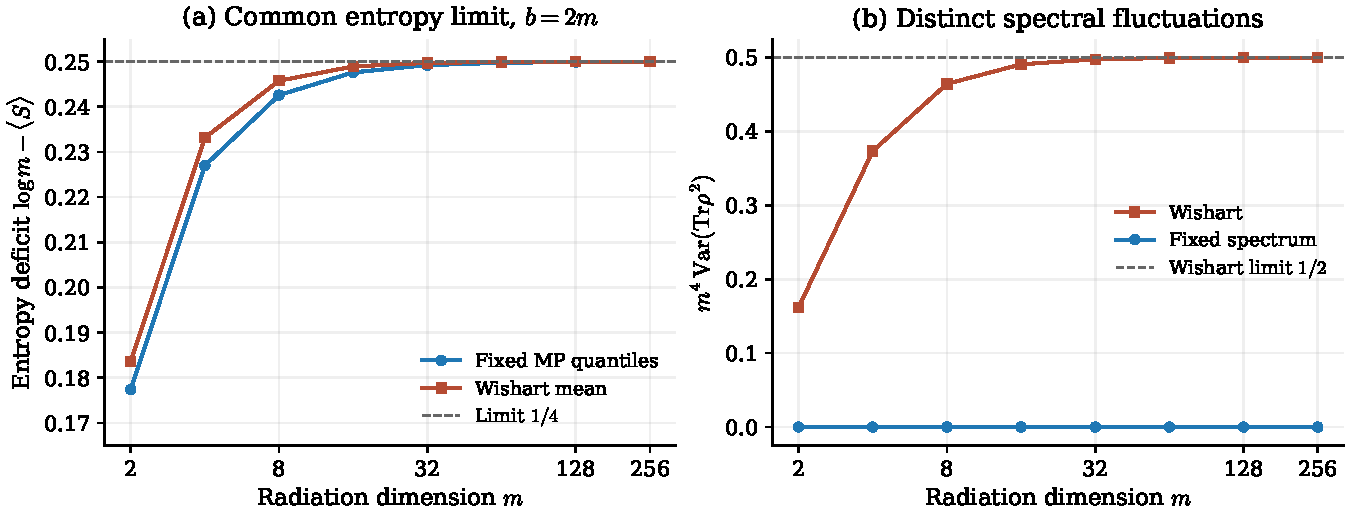
\includegraphics[width=\textwidth]{figures/output/fig05_ensemble_comparison.pdf}
 \caption{A common limiting entropy and different purity fluctuations.
 Left: the entropy deficit $\log m-S$ of the deterministic
 Marchenko--Pastur quantile spectrum and the exact mean deficit of the
 normalized Wishart ensemble, at $b=2m$.  Both tend to $1/4$.
 Right: the exact quantity $m^4\mathrm{Var}(\mathrm{Tr}\rho^2)$
 tends to $1/2$ for Wishart and is zero for the fixed spectrum.
 All curves are computed from the displayed quantiles and exact
 formulas; no fitted fluctuation profile is used.}
 \label{fig05:ensemble_comparison}
\end{figure}

\subsection{Information absent even from the complete spectrum}
\label{subsec05:level_one}

At finite dimension, knowledge of every power trace determines the
eigenvalues including multiplicities.  It still leaves the eigenvectors
undetermined.  For example, if $\Lambda$ is a nondegenerate diagonal
state and $V$ a unitary that mixes its eigenvectors, then $\Lambda$
and $V\Lambda V^\dagger$ have identical entropies of every R\'enyi
order.  Their expectation of a specified radiation observable $O$
need not agree:
\begin{equation}
\label{eq05:isospectral_observables}
 \mathrm{Tr}(O\Lambda)
 \ne\mathrm{Tr}(OV\Lambda V^\dagger)
\end{equation}
for a suitable $O$.  With $m=2$, $\Lambda=\mathrm{diag}(p,1-p)$,
$p\ne1/2$, and $V$ the Hadamard matrix, the expectation of the Pauli
operator $Z$ is $2p-1$ in the first state and zero in the second.
This exact example does not depend on a large-entropy approximation.

The choice of observable presupposes a physical basis or algebra of
radiation measurements.  Basis rotations are irrelevant when the task
is only to classify spectra, but they become relevant once couplings,
spatially localized operators, or a decoding map have been specified.
Even an exact entanglement spectrum is therefore an incomplete
specification of the radiation state.  Specifying a state at one time,
in turn, does not specify its dynamical map or its correlations with
other systems.  These are separate losses of information, and higher
spectral resolution repairs only the first of them.

\subsection{A conditional organization of observables}
\label{subsec05:level_three}
\label{subsec05:summary}

The preceding results suggest organizing comparisons by the data actually
being matched.  Table~\ref{tab05:hierarchy_summary} lists the additional
inputs needed at each stage.  This is an organization of questions,
rather than a theorem that all microscopic proposals must agree until
some predetermined order in entropy.  Two models can already disagree
in their leading density if their constraints or statistical weights
differ.  Conversely, their fluctuation statistics can agree within a
common universality class, so observing a variance does not automatically
identify a unique mechanism.

\begin{table}[htbp]
\centering
\caption{Information supplied by different comparisons.  Each row
requires its own assumptions; agreement in one row does not establish
agreement in the next.}
\label{tab05:hierarchy_summary}
\begin{adjustbox}{max width=\textwidth,center}
\begin{tabular}{p{0.23\textwidth}p{0.32\textwidth}p{0.35\textwidth}}
\toprule
Data compared & What can be inferred & Information still required\\
\midrule
Entropy at each time & Agreement of one scalar statistic & Spectrum,
reference correlations, and channel action\\
Limiting scaled spectrum & Leading integrable spectral statistics &
Finite-dimensional corrections and spectral covariance\\
Connected spectral moments & Fluctuations in a specified ensemble &
Eigenvectors and realization of that ensemble\\
Selected radiation--reference correlators & The specified input-dependent
correlations & Channel behavior beyond these correlators\\
\bottomrule
\end{tabular}
\end{adjustbox}
\end{table}

Thermodynamic averaging introduces a further specification: the joint
law of the fluctuating entropies or energies and their relation to the
radiation state.  Equality of dimensions or heat capacities does not
supply that law.  Section~\ref{sec04:paper_two_ensemble} describes
this dependence, while Section~\ref{sec06:annealed_quenched} treats
the distinction between averaged replica moments, spectral fluctuations,
and the entropy of an averaged density matrix.  Together with the
explicit comparison above, these distinctions state the limitations
of Page-curve matching without attributing uncomputed predictions to
individual proposals.

\section{R\'enyi averages and entropy fluctuations}
\label{sec06:annealed_quenched}

An ensemble-averaged Page curve specifies a mean entropy.  It does not
specify how much the entropy varies between realizations, or how the
radiation states themselves vary.  These questions require different
observables.  We first distinguish the two customary orders of averaging
R\'enyi entropies, then relate their difference to a normalized replica
covariance.  The identities are elementary at finite dimension, but their
normalization and order of limits are essential when applying them to a
gravitational replica calculation.

Throughout this section, $\rho$ is a random density matrix on a fixed
$d$-dimensional Hilbert space, normalized separately in every realization:
$\rho\geq0$ and $\tr\rho=1$ almost surely.  The probability measure may
describe random states, couplings, circuits, or another specified
preparation.  Its mathematical existence does not determine which of
these physical interpretations is appropriate.  Logarithms are natural,
and $0\log0=0$.

\subsection{The two R\'enyi averages}
\label{subsec06:why_matters}

For real $n>1$, define the moment $M_n(\rho)=\tr\rho^n$ and the
annealed and quenched R\'enyi entropies by
\begin{align}
 A_n&=\frac{\log\E M_n}{1-n},
 \label{eq06:annealed_def}\\
 Q_n&=\frac{\E\log M_n}{1-n}=\E S_n(\rho).
 \label{eq06:quenched_def}
\end{align}
The labels refer only to the position of the logarithm relative to the
average.  In particular, $Q_n$ is still an ensemble average, rather than
the entropy of a distinguished member.  Concavity of the logarithm gives
\begin{equation}
 G_n:=Q_n-A_n
 =\frac{\log\E M_n-\E\log M_n}{n-1}\geq0.
 \label{eq06:gap_def}
\end{equation}
At a fixed order $n>1$, equality holds precisely when $M_n$ is constant
almost surely.  Constancy of one moment neither fixes the spectrum nor
identifies a Hamiltonian.  Even constancy of every spectral moment leaves
the eigenvectors undetermined.

\begin{proposition}[Von Neumann limit and its first correction]
\label{prop06:von_neumann_limit}
For any ensemble of normalized density matrices on a common
finite-dimensional Hilbert space,
\begin{equation}
 \lim_{n\to1}A_n=\lim_{n\to1}Q_n=\E S(\rho),
 \qquad S(\rho)=-\tr(\rho\log\rho).
 \label{eq06:common_limit}
\end{equation}
Moreover, as $t\to0$,
\begin{equation}
 G_{1+t}=\frac{t}{2}\Var[S(\rho)]+O(t^2).
 \label{eq06:gap_formula}
\end{equation}
The remainder is bounded uniformly over ensembles at fixed dimension.
\end{proposition}

\begin{proof}
Set $L_2(\rho)=\tr[\rho(\log\rho)^2]$.  Expansion of the normalized
moment gives
\begin{equation}
 M_{1+t}=1-tS+\frac{t^2}{2}L_2+O(t^3),\qquad
 \log M_{1+t}=-tS+\frac{t^2}{2}(L_2-S^2)+O(t^3).
 \label{eq06:moment_expansion}
\end{equation}
For $n$ in a compact interval contained in $(0,\infty)$, the functions
$x^n|\log x|^r$, extended by zero at $x=0$, are uniformly bounded on
$[0,1]$.  Summing over at most $d$ eigenvalues bounds the required
moment derivatives uniformly, including for rank-deficient states.
The moment also has a positive lower bound near $n=1$, so the logarithm
has uniformly bounded derivatives there.  These facts justify averaging
the Taylor expansions.  The linear coefficients of $\log\E M_{1+t}$
and $\E\log M_{1+t}$ are both $-\E S$.  Their quadratic coefficients
differ by $\Var(S)/2$.  Dividing their difference by $t$ proves the
claim.
\end{proof}

Thus there is no nonzero annealed--quenched von Neumann entropy gap
under these definitions.  Entropy fluctuations survive as the slope
of the finite-order R\'enyi gap.  The statement holds for each finite
dimension.  A large-dimension saddle approximation followed by analytic
continuation may require additional uniform estimates; such an
approximation does not change the exact finite-dimensional identity.
For an infinite-dimensional state space, the interchange of derivatives
and averages must instead be justified by suitable integrability bounds.

\subsection{Averaging a spectrum and averaging a state}
\label{subsec06:state_average}

Another nonnegative difference, often relevant to ensemble
interpretations, is
\begin{equation}
 \chi=S(\bar\rho)-\E S(\rho),\qquad \bar\rho=\E\rho.
 \label{eq06:holevo_quantity}
\end{equation}
This is the Holevo quantity of the state ensemble.  It compares the
entropy of the averaged density operator with the mean entropy.  It
is not the $n\to1$ limit of $G_n$.  More explicitly,
\begin{equation}
 \chi=\E D(\rho\Vert\bar\rho),\qquad
 D(\rho\Vert\sigma)=\tr[\rho(\log\rho-\log\sigma)]\geq0,
 \label{eq06:relative_entropy_identity}
\end{equation}
where the support of $\rho$ lies in that of $\bar\rho$ almost surely.
Hence $\chi=0$ precisely when the density matrices themselves agree
almost surely.  This is a statement about the specified state ensemble,
not about whether an underlying theory is unique.

For comparison, let $\nu_\rho=\sum_{i=1}^d\delta_{\lambda_i(\rho)}$
be the eigenvalue counting measure.  Entropy is a linear functional of
this measure:
\begin{equation}
 -\int_0^1 x\log x\,\E\nu_\rho(dx)=\E S(\rho).
 \label{eq06:averaged_spectral_density}
\end{equation}
Averaging the spectral density before performing the entropy integral
therefore gives the mean entropy exactly.  The eigenvalues of
$\E\rho$ are generally not the averaged eigenvalue counting measure.
A concavity argument for density operators cannot be transferred to
this linear spectral integral.

An isospectral ensemble illustrates the distinction.  Fix a density
matrix $\rho_0$ and draw $\rho=U\rho_0U^\dagger$ with Haar-distributed
$U$.  All $M_n$, all R\'enyi entropies, and $S$ are deterministic, so
$G_n=0$ and $\Var(S)=0$.  Nevertheless $\bar\rho=I_d/d$ and
$\chi=\log d-S(\rho_0)$, which is positive unless $\rho_0$ is maximally
mixed.  For a pure $\rho_0$, $\chi=\log d$.  The radiation states can
therefore vary strongly while their entropies have no fluctuations at
all.  Conversely, a positive $G_n$ can arise from random preparation
within a fixed theory; it does not establish averaging over Hamiltonians.

\subsection{An exactly evaluated two-state ensemble}
\label{subsec06:two_state_example}

Consider the qubit ensemble
\begin{equation}
 \rho=\begin{cases}
 |0\rangle\langle0|,&\text{with probability }p,\\
 I_2/2,&\text{with probability }1-p,
 \end{cases}
 \qquad 0\leq p\leq1.
 \label{eq06:two_state_ensemble}
\end{equation}
Its moment has the two values $1$ and $2^{1-n}$.  All quantities in the
preceding discussion can therefore be calculated without a saddle
approximation:
\begin{align}
 Q_n&=(1-p)\log2,
 & A_n&=-\frac{\log[p+(1-p)2^{1-n}]}{n-1},
 \label{eq06:two_state_renyi}\\
 \Var(S)&=p(1-p)(\log2)^2,
 & \chi&=h_2\!\left(\frac{1+p}{2}\right)-(1-p)\log2,
 \label{eq06:two_state_variance}
\end{align}
where $h_2(x)=-x\log x-(1-x)\log(1-x)$ is binary entropy.
For $p=1/2$, the common von Neumann limit is $\log2/2$, whereas
$\chi=0.215762\ldots$.  At $n=2$,
$G_2=\log(3/4)+\log2/2=0.058892\ldots$.  The coefficient of $n-1$
in $G_n$ is $(\log2)^2/8=0.060057\ldots$.

\begin{figure}[htbp]
 \centering
 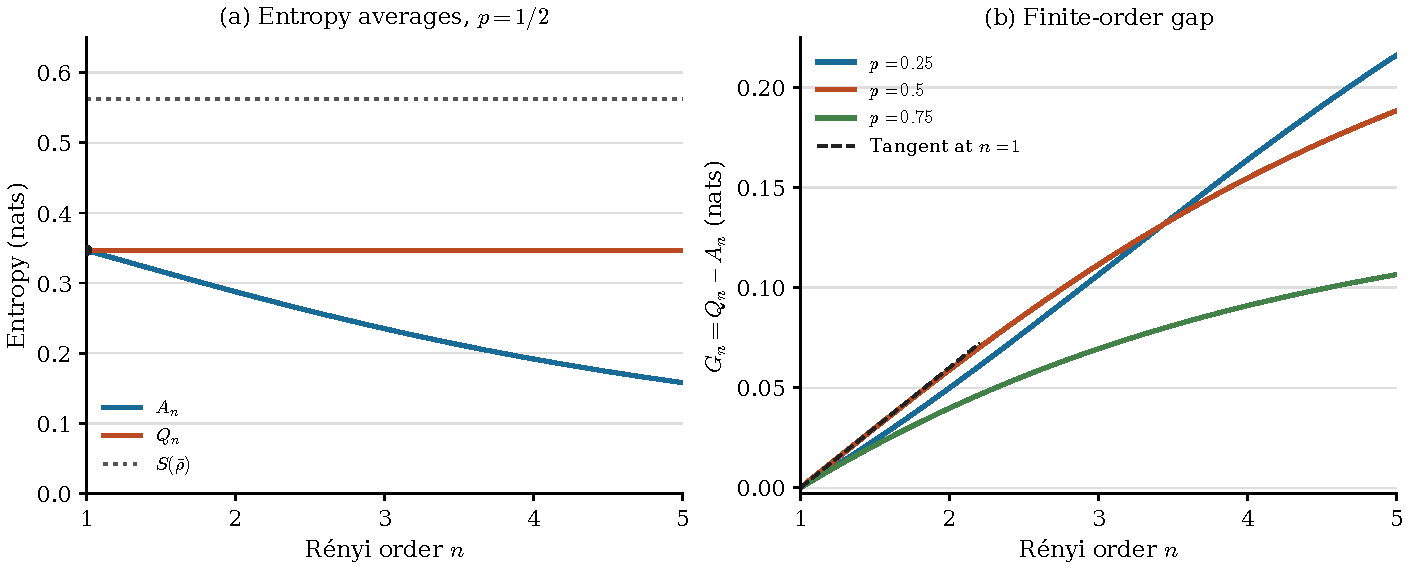
\includegraphics[width=\textwidth]{figures/output/fig06_renyi_gap.pdf}
 \caption{Exact averages for the qubit ensemble in
 \eqref{eq06:two_state_ensemble}.  Left: $A_n$ and $Q_n$ at $p=1/2$
 approach the same von Neumann limit; the entropy $S(\bar\rho)$ of the
 averaged state remains a different quantity.  Right: the nonnegative
 gap $G_n=Q_n-A_n$ for three mixing probabilities.  The dashed tangent
 at $p=1/2$ is $(n-1)\Var(S)/2$.  Every curve is obtained from
 \eqref{eq06:two_state_renyi}; no Page-time profile or gravitational
 fluctuation amplitude is assumed.}
 \label{fig06:annealed_quenched_gap}
\end{figure}

This example makes the observable distinction independent of any
large-entropy limit.  It also shows why the dependence of a fluctuation
observable on Page time cannot be inferred from Jensen's inequality.
The probability distribution and its time dependence would have to be
provided by a dynamical or state-preparation model.  A positive finite
R\'enyi gap, by itself, gives neither a universal peak position nor a
universal amplitude.

\subsection{Normalized replica covariances}
\label{subsec06:gap_computation}

The object that determines entropy fluctuations is the connected
moment
\begin{equation}
 C(n,\ell)=\E[M_nM_\ell]-\E M_n\,\E M_\ell.
 \label{eq06:connected_contrib}
\end{equation}
Normalization immediately implies $C(1,\ell)=C(n,1)=0$.  Differentiating
with respect to the two independent replica indices gives
\begin{equation}
 \left.\partial_n\partial_\ell C(n,\ell)\right|_{n=\ell=1}
 =\Var[S(\rho)].
 \label{eq06:entropy_covariance}
\end{equation}
Both identities are exact, with differentiation justified as in
Proposition~\ref{prop06:von_neumann_limit}.  The covariance contains
information absent from the one-point function $\E M_n$.  Knowing
the averaged spectral density, even exactly, does not determine it.

Proposition~\ref{prop05:exact_spectral_separation} gives an exact
finite-dimensional example of this separation.  Its two ensembles have
the same $\E M_n$ at every positive real order, the same mean entropy,
and the same averaged density matrix.  Consequently all their $A_n$
and their Holevo quantities agree.  One ensemble has a fixed spectrum,
whereas the other has two spectra with different entropies.  The latter
therefore has a nonzero entropy variance and a nonzero slope of $G_n$
at one.  Thus even complete knowledge of the one-point replica function
cannot reconstruct this fluctuation observable.

For a Haar-distributed pure state on $\mathbb C^m\otimes\mathbb C^b$,
let $\rho$ be the reduction to $\mathbb C^m$.  A useful exact comparison
is the purity variance~\citep{giraud2007}:
\begin{equation}
 \E M_2=\frac{m+b}{mb+1},\qquad
 C(2,2)=\frac{2(m^2-1)(b^2-1)}{(mb+1)^2(mb+2)(mb+3)}.
 \label{eq06:haar_purity_variance}
\end{equation}
Appendix~\ref{sec14:appendix_discrimination} derives this formula
from normalized replica contractions.  It vanishes if either subsystem
is one-dimensional and, for $m=b\to\infty$, is $2m^{-4}+O(m^{-6})$.
The finite normalization factors contribute at the leading order of
the covariance, even though they only correct the leading mean purity
at subleading order.  A product of one-point approximations is therefore
insufficient for computing this variance.

\subsection{Concentration and its limits}
\label{subsec06:self_averaging}

For a specified order $n>1$, concentration of $M_n$ controls $G_n$.
Write $M_n=\mu_n(1+\delta_n)$, where $\mu_n=\E M_n$ and
$\E\delta_n=0$.  If $|\delta_n|\leq\eta<1$ almost surely, Taylor's
theorem applied to $-\log(1+\delta_n)$ gives the two-sided bound
\begin{equation}
 \frac{\E\delta_n^2}{2(n-1)(1+\eta)^2}
 \leq G_n\leq
 \frac{\E\delta_n^2}{2(n-1)(1-\eta)^2}.
 \label{eq06:gap_bound}
\end{equation}
Under the same condition the quadratic approximation is
\begin{equation}
 G_n=\frac{\Var(M_n)}{2(n-1)\mu_n^2}
 +O\!\left(\frac{\E|\delta_n|^3}{(n-1)(1-\eta)^3}\right).
 \label{eq06:relative_variance_expansion}
\end{equation}
These estimates state an explicit condition controlling the logarithm.
A small relative variance alone does not uniformly control rare events
with $M_n/\mu_n$ very close to zero as the dimension increases.  At
fixed dimension the lower bound $M_n\geq d^{1-n}$ supplies a bound,
but its constant need not remain useful in a large-dimension limit.

Near $n=1$, the numerator in the leading term of
\eqref{eq06:relative_variance_expansion} itself vanishes quadratically:
$\Var(M_{1+t})=t^2\Var(S)+O(t^3)$.  This restores the linear behavior
in \eqref{eq06:gap_formula}; treating that numerator as independent of
$n$ would give a spurious singularity.  Separately, an entropy variance
bound has the direct probabilistic consequence
\begin{equation}
 \Prob\{|S-\E S|\geq a\}\leq\frac{\Var(S)}{a^2},\qquad a>0.
 \label{eq06:entropy_concentration}
\end{equation}
This controls deviations of the entropy at the specified preparation
or time.  It does not imply concentration of the density operator, nor
simultaneous agreement of an entire trajectory without further temporal
control.

\subsection{Fluctuations within and between preparations}
\label{subsec06:conditional_variance}

An ensemble may contain more than one source of randomness.  Let
$\Theta$ denote a classical preparation parameter, such as an energy
window or the number of available environment states.  The law of total
variance gives
\begin{equation}
 \Var(S)=\E\bigl[\Var(S\mid\Theta)\bigr]
       +\Var\bigl(\E[S\mid\Theta]\bigr).
 \label{eq06:total_variance}
\end{equation}
The first term describes entropy fluctuations with the preparation held
fixed; the second describes variation of the conditional mean between
preparations.  They need not have the same size or the same dependence
on subsystem dimensions.  Matching one of these terms between models
does not match their total variance.

For example, keep the radiation dimension $m$ fixed and draw a positive
integer environment dimension $B$ from a specified distribution.
Conditional on $B=b$, draw a Haar bipartite state on
$\mathbb C^m\otimes\mathbb C^b$.  Every reduced state acts on the
same radiation Hilbert space, so the preceding finite-dimensional
identities apply even though the purifying space varies.  The exact
purity variance is
\begin{align}
 \Var(M_2)
 &=\E\!\left[
 \frac{2(m^2-1)(B^2-1)}{(mB+1)^2(mB+2)(mB+3)}\right]
 \notag\\
 &\quad+\Var\!\left(\frac{m+B}{mB+1}\right).
 \label{eq06:random_dimension_variance}
\end{align}
The second term is absent in a fixed-dimension comparison.  This
example supplies a precise probabilistic distinction between state
fluctuations at fixed dimension and fluctuations of the available number
of states.  It does not identify an arbitrary gravitational ensemble
with a mixture of Haar ensembles; that identification would require
the conditional state law as well as the distribution of $B$.

Conditioning also clarifies how thermodynamic broadening and entropy
fluctuations enter a comparison.  A fluctuating energy can change the
conditional mean entropy, while states within a narrow energy window
can still have a nonzero conditional variance.  A measured or computed
total variance alone cannot separate these contributions.  The
preparation or conditioning must be stated before assigning a physical
origin to either term.  All statements here concern a classical
probability distribution over density operators; replacing it by a
coherent superposition is a different state construction.

\subsection{Application to gravitational ensembles}
\label{subsec06:interpretation}

When a path integral initially constructs an unnormalized positive
operator $W$, the physical moment is
\begin{equation}
 M_n=\frac{\tr W^n}{(\tr W)^n}.
 \label{eq06:normalized_ratio}
\end{equation}
The average of this ratio generally differs from replacing its
denominator by $(\E\tr W)^n$.  In a covariance calculation, fluctuations
of the normalization can enter at the same order as the connected
numerator.  The normalization check $C(1,\ell)=0$ must hold before
using a replica derivative to infer entropy fluctuations.

Bousso and Miyaji~\citep{boussomiyaji2024} computed such fluctuations
in the PSSY model, explicitly retaining the fluctuating normalization.
Their calculation includes non-tubular and tubular contributions and
finds a difference from fixed-dimension Haar fluctuations after the
Page time, associated with fluctuations of the number of black hole
states in the chosen energy window.  This is an existing example of
information beyond the mean Page curve.  It is not a nonzero difference
between the two normalized von Neumann limits in
\eqref{eq06:common_limit}.  Moreover, connected replica geometries
need not introduce a handle: connectivity and genus are distinct
properties, and the suppression of a covariance must be calculated
in the specified model.

For a comparison between microscopic proposals, the ensemble measure,
normalization prescription, state preparation, and observable must
therefore be held fixed or related explicitly.  A nonzero covariance
can distinguish two specified preparations with different fluctuations.
Neither its presence nor its absence alone decides whether gravity is
described by one Hamiltonian.  The finite R\'enyi gap and entropy variance
provide useful additional data, while leaving the separate question of
recovering an unknown input to a channel analysis.

\section{Comparisons between gravitational descriptions}
\label{sec07:discriminating}

The examples above show that a radiation entropy, an averaged spectrum,
a fluctuation, and a channel recovery test answer different questions.
Applying these comparisons to gravity requires specifying the models
on both sides. The broad names used for approaches to the information
problem do not supply complete microscopic ensembles or evaporation
maps. They can also refer to different parts of one description:
a microscopic Hamiltonian, a family of states, a semiclassical
calculation, or a prescription for interior operators.

\subsection{What an entropy calculation establishes}

A calculation of $S(R)$ in a specified state constrains that state's
reduced density matrix. In gravity, the island prescription additionally
relates the entropy to a generalized-entropy extremization problem
\cite{engelhardtwall2015,penington2020,almheirietal2019}.
When accompanied by a code-subspace description and suitable
reconstruction assumptions, the calculation can support conclusions
about recoverable interior observables. Ref.~\cite{pssyetal2022}
contains an explicit Petz-map reconstruction argument in addition to
its replica entropy computation. These additional structures are not
encoded in the scalar function $S(R)$ alone.

This distinction prevents two opposite inferences. An entropy curve
that agrees with a unitary random-state benchmark does not uniquely
identify its preparation. Conversely, the existence of elementary
replacement-channel examples does not invalidate a reconstruction
argument that supplies more information than that curve. The examples
in section~\ref{sec02:page_curve_establishes} hold the specified
radiation data fixed while changing the channel on other inputs. A
gravity calculation that determines those additional inputs or their
reference correlations can exclude the replacement channel.

Matching the full sequence $\E\mathrm{Tr}\rho_R^n$ likewise has a
precise meaning. At fixed dimension it determines the averaged spectral
measure, since that measure is supported on a compact interval. It
does not determine a probability law on spectra. The finite-dimensional
construction in section~\ref{sec16:exact_ensembles} demonstrates
this difference without an asymptotic approximation. A two-trace
correlator supplies additional data. Even those spectral data leave
operator matrix elements and the input dependence of the channel
unspecified.

\subsection{The objects supplied by different approaches}

\paragraph{Random-state and random-circuit models.}
A Haar-induced state is a precisely defined statistical model. It gives
finite-dimensional moments and fluctuations once the dimensions and
symmetry class are fixed. A random circuit can also specify an actual
channel and a time parameter. Its circuit architecture, depth, and
required design order then affect the approach to a design
\cite{brandaoetal2016}.
Replacing a circuit by a Haar state at every time retains a useful
benchmark but discards information about the temporal coupling of the
states. Section~\ref{sec08:equilibrium_evaporation} makes that distinction
explicit.

\paragraph{Islands and replica wormholes.}
An island calculation is a prescription for entropies and related
observables within a gravitational setup. In the model of
ref.~\cite{pssyetal2022}, the replica sum can be compared with a
random-state spectral problem. In JT gravity, the matrix-integral
description computes particular ensemble quantities
\cite{saadetal2019}. Neither statement implies that every island
calculation is an ensemble of the same microscopic Hamiltonians.
Whether a boundary description is fixed or ensemble averaged is a
question about its definition and factorization properties
\cite{marolfmaxfield2020}. It cannot be settled by a von Neumann
annealed--quenched gap under the normalized definitions of
section~\ref{sec06:annealed_quenched}, because that gap vanishes.

\paragraph{Microstate geometries and the fuzzball program.}
Microstate constructions seek a microscopic description of black-hole
states and their effective geometric properties. Mathur's analysis also
emphasizes restrictions on attempts to restore purity through small
corrections to a specified pair-creation process \cite{mathur2009}.
A radiation-spectrum comparison requires a chosen family of states,
a probability distribution if an average is taken, and a coupling to
the radiation. The name of the program alone does not determine an
entanglement-spacing distribution or an entropy variance. In
particular, a claim about integrability of a Hamiltonian does not by
itself provide the local statistics of the reduced density matrix
produced in a specified evaporation experiment.

\paragraph{State-dependent interior operators.}
State-dependent constructions concern the map between boundary
observables and interior operators in a specified class of states
\cite{papadodimasraju2014}. To compare them through outgoing radiation,
one must identify a boundary preparation and an observable whose
prediction differs. A different representation of interior operators
need not change the radiation density matrix. If the same microscopic
state and outgoing algebra are used, all radiation entropies can agree
without resolving how the interior is represented.

\paragraph{Geometric descriptions of entanglement.}
The ER=EPR proposal relates entanglement to geometric connections
\cite{maldacenasusskind2013}. By itself it does not specify a normalized
probability law for Hawking-radiation density matrices. A spectral or
recovery comparison therefore requires a concrete realization of the
proposal and a common set of observables. Its statements can coexist
with a microscopic unitary theory and with a semiclassical island
calculation. Treating these descriptions as mutually exclusive rows
with independently fixed numerical predictions would impose more
structure than their names provide.

\subsection{A comparison table with explicit status}

Table~\ref{tab07:comparisons} collects calculations rather than assigning
uncomputed predictions to broad programs. An equality in one row does
not imply equality in another. In particular, the energy ensemble and
accessible algebra must be held fixed in a channel comparison, while
normalization and matrix dimensions must be held fixed in a spectral
comparison.

\begin{table}[tbp]
\centering
\caption{Specified comparisons and the information they add. The first
four rows are calculated examples in this paper. The final two identify
gravity calculations from the literature or further model-dependent
questions; they are not predictions shared by every member of a named
approach.}
\label{tab07:comparisons}
\begin{adjustbox}{max width=\textwidth,center}
\begin{tabular}{p{0.24\textwidth}p{0.31\textwidth}p{0.35\textwidth}}
\toprule
Comparison & Data that agree & Additional distinction \\
\midrule
Isometry and replacement channel & All radiation states for one input
& Reference mutual information and recovery fidelity differ exactly \\[4pt]
Finite spectral ensembles & Averaged replica moments at every order
and mean entropy & Purity and entropy covariances differ exactly \\[4pt]
Fixed MP quantiles and Wishart states & Limiting density and mean
entropy correction & Fixed versus fluctuating purity at finite dimension \\[4pt]
Gaussian and quartic branch differences & Mean and variance & Central
deficit and full averaged-minimum profile differ \\[4pt]
Gravitational entropy fluctuations & A specified mean Page curve
& Connected normalized replicas give model-dependent fluctuations;
ref.~\cite{boussomiyaji2024} computes an example \\[4pt]
Two proposed microscopic evaporation models & To be established for the
chosen states and couplings & Compute a common operator, reference, or
covariance observable before asserting a difference \\
\bottomrule
\end{tabular}
\end{adjustbox}
\end{table}

The last row is a research requirement. It is not an inference that all
microscopic descriptions must eventually disagree on one of the listed
quantities. Distinct descriptions of the same physics can agree on all
accessible observables. Conversely, two models can already differ in a
leading entropy curve if their state preparation, constraints, or
dynamics differ. There is no general rule that physically meaningful
differences begin only at a particular genus order.

\subsection{Precision, normalization, and accessible observables}

Three quantitative checks are needed before a small difference becomes
a useful comparison. First, the error of each calculation must be
smaller than the proposed distinction. Leading convergence to a common
spectral density does not control a finite-size covariance; the Haar
purity example illustrates the normalization terms required at that
order. Second, the same ensemble operation must be computed on both
sides. A ratio of averaged partition functions can differ from an
average of normalized density-matrix moments. Third, the observable
must belong to the algebra accessible in the proposed experiment.
An operator involving an external reference requires that reference
to be part of the state preparation.

Ensemble variance also differs from quantum measurement variance in a
single member. For an observable $O$ and states $\rho_\alpha$, the
variance in the average state decomposes as
\begin{align}
 \mathrm{Tr}(\overline\rho O^2)
 -\bigl[\mathrm{Tr}(\overline\rho O)\bigr]^2
 &=\E_\alpha\left[\mathrm{Tr}(\rho_\alpha O^2)
       -\mathrm{Tr}(\rho_\alpha O)^2\right]
 \nonumber\\
 &\quad+\Var_\alpha\left[\mathrm{Tr}(\rho_\alpha O)\right],
 \qquad \overline\rho=\E_\alpha\rho_\alpha.
 \label{eq07:variance_decomposition}
\end{align}
The two terms refer to repeated measurement within a preparation and
to variation between preparations. Determining which variation a
connected gravitational quantity represents requires an interpretation
of the ensemble. A single fixed Hamiltonian can still support an
ensemble of input states, random couplings in an experiment, or time
samples. A nonzero variance is therefore not, by itself, evidence for
an ensemble of Hamiltonians.

\section{From equilibrium states to evaporation dynamics}
\label{sec08:equilibrium_evaporation}

Equilibrium distributions and instantaneous random-state models give
well-defined entropy calculations. An evaporation process additionally
specifies how successive radiation subsystems arise from one evolution.
This distinction applies in AdS coupled to an absorbing bath as well as
in asymptotically flat settings. Dynamical island calculations already
study time-dependent evaporation
\citep{almheirietal2019,almheirietal2020page}; the issue here is which
additional assumptions permit the equilibrium and random-state
calculations of the preceding sections to describe such a history.

\subsection{Consistency of successive radiation states}
\label{subsec08:nested_channels}

Use the finite-dimensional notation of
Section~\ref{sec02:page_curve_establishes}. A sequential isometric model
has maps
\begin{equation}
\begin{aligned}
 U_k&:A\longrightarrow B_k\otimes R_k,\qquad
 W_{k+1}:B_k\longrightarrow B_{k+1}\otimes b_{k+1},\\
 U_{k+1}&=(W_{k+1}\otimes I_{R_k})U_k,
\end{aligned}
 \label{eq08:sequential_isometries}
\end{equation}
with the tensor factors reordered where necessary. Ancillas in a
specified initial state may be included in $B_k$. The corresponding
radiation channels $\Ncal_k(X)=\tr_{B_k}(U_kXU_k^\dagger)$ obey
\begin{equation}
 \tr_{b_{k+1}}\Ncal_{k+1}(X)=\Ncal_k(X)
 \quad\hbox{for every input operator }X.
 \label{eq08:channel_consistency}
\end{equation}
This equation assumes that emitted modes are no longer acted upon;
equivalently, their freely evolving observables can be described in an
interaction picture. It is a constraint on channels and their joint
outputs, not merely on the values of their entropies.

For example, assigning $|0\rangle\langle0|$ to the first emitted qubit
and a Bell state to the first two emitted qubits gives two valid
density matrices, both pure. They cannot be the successive radiation
states of this model: tracing the second qubit out of the Bell state
gives $I/2$, not $|0\rangle\langle0|$. Sampling an unrelated Haar state
at each instant similarly does not establish
equation~\eqref{eq08:channel_consistency}. A dynamical random-state
approximation must explain how the jointly distributed states are
generated, even when each individual state has the expected marginal
statistics. The constructions in
Proposition~\ref{prop02:channel_counterexample} do satisfy this
consistency condition because they release subsystems of a single
prepared output.

Entropy inequalities give a weaker, useful necessary condition. Since
$R_{k+1}=R_kb_{k+1}$,
\begin{equation}
 S(R_{k+1})-S(R_k)=S(b_{k+1}|R_k),\qquad
 |S(R_{k+1})-S(R_k)|\leq\ln\dim b_{k+1}.
 \label{eq08:entropy_increment}
\end{equation}
The bound follows from subadditivity and the Araki--Lieb inequality.
A decreasing radiation entropy requires negative conditional entropy
of the new emission given the earlier radiation. In the Bell-pair
example, the increment is $+\ln2$ for the first $q$ emissions and
$-\ln2$ for the last $q$. This accounts for the turnover through
explicit early--late correlations, while remaining insufficient to
decide whether those correlations encode the initial input.

\subsection{Fixed total energy does not fix the black-hole energy}
\label{subsec08:energy_constraints}

Energy conservation constrains the joint state rather than assigning
zero variance to the energy of every subsystem. For subsystems described
by an additive Hamiltonian, a fixed-total-energy space has the
decomposition
\begin{equation}
 \Hcal_{E_{\mathrm{tot}}}
 =\bigoplus_E\Hcal_B(E)\otimes
                  \Hcal_R(E_{\mathrm{tot}}-E).
 \label{eq08:energy_shell}
\end{equation}
A state in this space can have an arbitrary distribution $p_E$ over
the allowed black-hole energies. Orthogonality of the radiation energy
sectors makes its reduced state block diagonal,
\begin{equation}
 \rho_B=\bigoplus_Ep_E\rho_{B,E},\qquad
 S(\rho_B)=-\sum_Ep_E\ln p_E+
                     \sum_Ep_E S(\rho_{B,E}).
 \label{eq08:sector_entropy}
\end{equation}
The first term is the entropy of the energy-sector probabilities, and
the second is the mean entropy within sectors. Neither is fixed by
specifying $E_{\mathrm{tot}}$ alone. Sampling assumptions and dynamics
determine $p_E$.

The simplest illustration uses two qubits with excitation energy
$\varepsilon$. The pure state
\begin{equation}
 |\psi_p\rangle
 =\sqrt p\,|1\rangle_B|0\rangle_R
  +\sqrt{1-p}\,|0\rangle_B|1\rangle_R
 \label{eq08:fixed_energy_example}
\end{equation}
has exact total energy $\varepsilon$, but
\begin{equation}
 \Var(E_B)=\varepsilon^2p(1-p),\qquad
 S(\rho_R)=-p\ln p-(1-p)\ln(1-p).
 \label{eq08:fixed_energy_variance}
\end{equation}
These are quantum fluctuations in one pure state; no average over
Hamiltonians is involved. In an evaporating system, uncertainty in the
remaining energy can likewise be correlated with the energy already
emitted. Isolation does not justify replacing that distribution by a
delta function at the mean black-hole energy.

The equilibrium counterpart further specifies the distribution. If
states in a narrow total-energy shell are sampled with microcanonical
weights, then the energy-sector probabilities are proportional to the
product of the two densities of states. The stable quadratic expansion
of this product, derived in Section~\ref{sec04:paper_two_ensemble},
gives a variance of $E_B/T$ equal to the effective heat capacity
$(C_B^{-1}+C_R^{-1})^{-1}$. Fixing $E_B$ itself removes this exchange
fluctuation, whereas fixing $E_B+E_R$ does not. Because the two
subsystem energies are anticorrelated, the variance of the difference
between their thermodynamic entropies is four times the individual
entropy variance at leading Gaussian order~\citep{wuebben2026b}.
These thermodynamic entropies count states; they are distinct from
the fine-grained entropies in equation~\eqref{eq08:sector_entropy}.
An outgoing flux need not be in equilibrium with the remaining black
hole, so the equilibrium law cannot be assigned to evaporation without
justifying its exchange and sampling assumptions.

\subsection{A fluctuation width is not an evaporation timescale}
\label{subsec08:instantaneous_approximation}

Replacing an equilibrium parameter by a function of time does not
determine either the radiation channel or its preparation law.
Suppose, more specifically, that an instantaneous approximation has
identified two entropy branches with mean difference $\Delta(t)$ and
a distribution for their centered difference. Let its width in entropy
units be $\sigma_\Delta(t)$, and assume that the distribution and the
local entropy formula vary slowly while $\Delta(t)$ crosses zero.
If $\dot\Delta(t_*)\ne0$, linearization supplies the estimate
\begin{equation}
 \tau_{\mathrm{round}}\sim
 \frac{\sigma_\Delta(t_*)}{|\dot\Delta(t_*)|},
 \qquad \Delta(t_*)=0.
 \label{eq08:time_width}
\end{equation}
Its coefficient depends on the convention used to define a crossover
width. The estimate requires the fluctuation law and
$\dot\Delta$ to change little over $\tau_{\mathrm{round}}$; it also
requires relaxation to justify the instantaneous description. If the
crossing is tangent or relaxation is slow, the linear estimate fails.
A thermodynamic variance alone supplies none of these dynamical
conditions.

Similarly, a Marchenko--Pastur law at a fixed dimension ratio follows
from a stated random-state or covariance model, not from time
dependence of the ratio. Emission spectra, conserved charges and
energy-dependent matrix elements can change the allowed states and
their weights. In a gravitational application the relevant entropy
branches must be derived from the generalized entropy prescription;
they cannot always be replaced by logarithms of unweighted Hilbert
space dimensions. The calculations of
Sections~\ref{sec03:paper_one_universality} and
\ref{sec04:paper_two_ensemble} then provide conditional local models
whose assumptions can be tested in the dynamical setting. They do
not imply a universal sharp transition for isolated evaporation.

\subsection{What a dynamical comparison should specify}
\label{subsec08:dynamical_target}

A comparison between two evaporation models should fix the input
space, the preparation, the emitted radiation algebra, and the
conservation laws. It should state whether averages concern initial
states, dynamics, or Hamiltonians, and identify any degrees of freedom
that are traced out at the endpoint. Within that common setup, one
can compare radiation moments at specified times, their connected
fluctuations, and correlations between emissions. Reference-assisted
recovery tests then address the dependence on unknown inputs, as in
Section~\ref{subsec02:reference_test}. Computational difficulty of a
decoder is a further question beyond its mathematical existence
\citep{haydenpreskill2007}.

The gravitational calculation has additional responsibilities: a
specified coupling to a bath or asymptotic radiation region, a
semiclassical state and its backreaction, and a justification of the
entropy prescription in the regime being studied. These conditions
are realized to different degrees in existing island models
\citep{almheirietal2019,almheirietal2020page,almheirietal2020review}.
They should be evaluated model by model. Neither a fixed Hamiltonian
nor fixed total energy eliminates all statistical fluctuations, and
agreement of time-indexed equilibrium entropies does not establish
agreement of quantum channels. These distinctions specify the
additional calculations needed to connect the controlled examples in
this paper to microscopic black-hole information recovery.

\section{Further calculations}
\label{sec09:research_program}

The explicit examples leave several concrete questions for gravitational
models. Their resolution requires the following model-specific
calculations.

\subsection{Normalized two-trace fluctuations in a common preparation}

The most direct extension of a computed mean Page curve is a connected
correlator of normalized moments. One should specify the state
preparation, energy window, boundary conditions, and random variables
being averaged, then compute
\begin{equation}
 C(n,\ell)=\E[\mathrm{Tr}\rho_R^n\,\mathrm{Tr}\rho_R^\ell]
       -\E[\mathrm{Tr}\rho_R^n]\E[\mathrm{Tr}\rho_R^\ell].
 \label{eq09:covariance_target}
\end{equation}
The conditions $C(1,\ell)=C(n,1)=0$ are useful exact normalization
checks. Differentiation at $(1,1)$ gives the entropy variance when the
limits are justified. The calculation of ref.~\cite{boussomiyaji2024}
provides a gravitational example and a comparison with Haar-state
fluctuations. Extending this comparison to another specified
preparation would test how much of the covariance survives changes in
the energy window, state-count fluctuations, or bath coupling.

The finite spectral construction in
section~\ref{sec16:exact_ensembles} makes the missing information
precise: even all one-trace averaged moments leave a two-trace
covariance undetermined. A leading spectral calculation therefore
cannot replace this step. On the other hand, the covariance may itself
be shared by several models. Establishing a difference requires its
explicit value and controlled errors.

\subsection{Generalized-entropy response near a critical point}

The quartic thermodynamic law of Paper~II suggests a calculation in a
charged gravitational model with an actual entropy transition. First
locate the competing generalized-entropy branches for the chosen state
and radiation region. Next compute their joint response to the critical
mode, including the covariance of the area and bulk-entropy terms.
The relevant coefficient is the response of their difference, as in
\eqref{eq04:response}. A cancellation at that order would remove the
$N^{3/4}$ contribution even though each branch fluctuates on that scale.

A finite bath then changes the fluctuation law through its entropy
curvature. The $C_R\sim N^{3/2}$ crossover concerns the canonical
critical model and its stated reservoir regularity assumptions. A
physical application must check that the bath samples the required
energy range and that remote configurations do not dominate the entropy
moments. Finally, relaxation and evaporation times must be compared
before interpreting the equilibrium distribution as a time-dependent
radiation profile. These requirements make a critical enhancement a
conditional prediction that can be tested in a chosen setup.

\subsection{Spectral comparisons with matched conservation laws}

The Wishart benchmark has no energy constraint. A useful next model
would impose a common sector decomposition on both ensembles being
compared, match the sector probabilities and dimensions, and evaluate
both within-sector and between-sector fluctuations. For orthogonal
radiation sectors, the entropy is
$H(p)+\sum_\alpha p_\alpha S(\rho_{R,\alpha})$.
Fluctuating sector probabilities introduce covariance terms absent from
a fixed-dimension Haar calculation. Matching only the total dimension
would miss them.

Such a construction would also clarify when the canonical planar
correction of Paper~I can enter a comparison. When radiation resolves
the sector, the direct-sum identity applies; when sector contributions
overlap in the radiation space, a spectral calculation is needed.
One should determine this algebraic distinction from the state before
choosing a random-matrix approximation. It need not be a small
correction to the same model.

\subsection{Reference correlations and recovery}

A channel comparison can begin with a finite code subspace and an input
entangled with a reference. The target quantities include
$I(Q:R_t)$, the complementary correlations with the remaining black
hole, and the error of a specified recovery map. These quantities
address transfer of unknown quantum information, as in the decoding
perspective of Hayden and Preskill \cite{haydenpreskill2007}. They also
permit a direct comparison with reconstruction statements associated
with islands \cite{penington2020,pssyetal2022}.

A successful calculation should separate existence of a recovery map
from the resources needed to implement it. An isometry has a perfect
inverse on its image, but this fact gives no efficient circuit for
that inverse. Conversely, a complicated decoder does not imply that
the entropy curve is wrong. The chosen code subspace, accessible
radiation algebra, and permitted operations determine the operational
question.

\subsection{Reproducibility of the worked comparisons}

The figures in this paper are evaluated from the specified probability
laws and finite-dimensional formulas. They contain no fitted gravity
predictions. The accompanying calculations enumerate Haar permutations,
check the finite spectral examples, compare direct quadrature with
closed fluctuation profiles, and evaluate the fixed-quantile sequence.
The algebraic arguments establish the identities and limits; the
numerical checks test their implementations and finite-size values.
The figure programs and their dependencies are preserved with the
source.\footnote{Reproduction commands are listed in the project build
instructions. The computation programs are stored alongside the figure
programs, with exact permutation checks separated from numerical
quadrature.}

\section{Conclusion}
\label{sec10:conclusion}

A Page curve constrains radiation entanglement, while identifying an
information-recovery process requires information about the state
preparation and channel. The distinction can be made exact. An
isometry and a replacement channel reproduce every radiation state
along one chosen preparation, although they have different reference
correlations. Two finite-dimensional ensembles reproduce all averaged
replica moments and the same mean von Neumann entropy, although their
entropy fluctuations differ. Fixed Marchenko--Pastur spectra and
Wishart spectra provide a corresponding comparison in the usual
large-dimension regime.

These examples also identify quantities worth computing. Normalized
two-trace correlations determine entropy fluctuations through a mixed
replica derivative. The finite-order quenched-minus-annealed R\'enyi
gap vanishes at order one, with a slope set by half the entropy
variance. Entropy of an averaged state is a separate quantity. Keeping
these operations distinct is necessary when comparing a gravitational
path integral with an ensemble or a fixed preparation.

Thermodynamic broadening supplies additional information once the
competing branches and their joint law are specified. Equal variances
can give different crossover shapes, and a known fixed-law
averaged-minimum profile can determine its scalar fluctuation
distribution. Energy constraints, reservoir size, and cancellation of
a common mode determine how that distribution enters a radiation
entropy. A static distribution still requires an evolution law before
it becomes an evaporation prediction.

The remaining gravitational question is therefore model specific:
which additional spectral, operator, or reference-correlation data are
fixed by the proposed description, and which predictions differ under
a common preparation? Answering it would connect agreement with a Page
curve to a more complete account of information recovery.

\appendix
\section{Review of Free Probability and Non-Crossing Partitions}
\label{sec11:appendix_free_prob}

This appendix provides a self-contained summary of the free-probability
tools used throughout the paper.  The target reader is an
information-paradox researcher who is familiar with random-matrix theory
at the level of Wishart ensembles but has not encountered the
combinatorial framework of free probability.  Comprehensive treatments
can be found in Nica and Speicher~\cite{nicaspeicher2006} and in the
foundational papers of Voiculescu~\cite{voiculescu1991} and
Speicher~\cite{speicher1994}.

\subsection{Non-crossing partitions}
\label{subsec11:non_crossing}

Let $[n] = \{1,2,\ldots,n\}$.  A \emph{partition} $\pi$ of $[n]$ is a
collection of non-empty, pairwise disjoint subsets (called \emph{blocks})
whose union is $[n]$.  The set of all partitions of $[n]$ is denoted
$\mathcal{P}(n)$.

A partition $\pi \in \mathcal{P}(n)$ is \emph{non-crossing} if there do
not exist elements $a < b < c < d$ in $[n]$ such that $a,c$ belong to
one block and $b,d$ belong to a different block.  Equivalently, when the
elements of $[n]$ are arranged around a circle, the convex hulls of the
blocks do not intersect.  The set of non-crossing partitions of $[n]$ is
denoted $\mathrm{NC}(n)$.

\paragraph{Small examples.}
For $n=1$ there is a single partition $\{\{1\}\}$, which is non-crossing.
For $n=2$ there are two partitions, $\{\{1\},\{2\}\}$ and
$\{\{1,2\}\}$; both are non-crossing.  For $n=3$ there are five
partitions: $\{\{1\},\{2\},\{3\}\}$, $\{\{1,2\},\{3\}\}$,
$\{\{1,3\},\{2\}\}$, $\{\{1\},\{2,3\}\}$, and $\{\{1,2,3\}\}$.  All
five are non-crossing.  For $n=4$ there are $15$ partitions in total, of
which exactly $14$ are non-crossing; the sole crossing partition is
$\{\{1,3\},\{2,4\}\}$.

\paragraph{Lattice structure.}
The set $\mathrm{NC}(n)$, ordered by refinement (i.e.\ $\pi \leq \sigma$
if every block of $\pi$ is contained in a block of $\sigma$), forms a
lattice: any two elements have a unique meet and join.  This lattice is
self-dual and graded, with the rank of $\pi$ equal to $n$ minus the
number of blocks~\cite{nicaspeicher2006}.

\subsection{Catalan numbers}
\label{subsec11:catalan}

The cardinality of $\mathrm{NC}(n)$ is the $n$-th Catalan number:
\begin{equation}
\label{eq11:catalan}
  C_n
  \;=\;
  \bigl|\mathrm{NC}(n)\bigr|
  \;=\;
  \frac{1}{n+1}\binom{2n}{n}\,.
\end{equation}
The first several values are
\begin{equation}
\label{eq11:catalan_values}
  C_1 = 1,\quad
  C_2 = 2,\quad
  C_3 = 5,\quad
  C_4 = 14,\quad
  C_5 = 42,\quad
  C_6 = 132\,.
\end{equation}
The generating function is
\begin{equation}
\label{eq11:catalan_gf}
  C(z)
  \;=\;
  \sum_{n=0}^{\infty} C_n\, z^n
  \;=\;
  \frac{1 - \sqrt{1 - 4z}}{2z}\,,
\end{equation}
satisfying the quadratic relation $C(z) = 1 + z\,C(z)^2$.  The
asymptotic growth is
\begin{equation}
\label{eq11:catalan_asymp}
  C_n
  \;\sim\;
  \frac{4^n}{n^{3/2}\sqrt{\pi}}
  \qquad
  (n \to \infty)\,.
\end{equation}

For comparison, the total number of partitions of $[n]$ is the Bell
number $B_n$, which grows much faster: $B_4 = 15$, $B_5 = 52$,
$B_6 = 203$.  The distinction between $C_n$ and $B_n$ is the
combinatorial signature of the difference between free and classical
probability.

\subsection{Narayana numbers}
\label{subsec11:narayana}

The Catalan number $C_n$ counts all non-crossing partitions of $[n]$
without regard to the number of blocks.  A finer count is provided by
the Narayana numbers:
\begin{equation}
\label{eq11:narayana}
  N(n,k)
  \;=\;
  \frac{1}{n}\binom{n}{k}\binom{n}{k-1}\,,
  \qquad
  k = 1, 2, \ldots, n\,,
\end{equation}
which count the number of non-crossing partitions of $[n]$ with exactly
$k$ blocks.  They satisfy
\begin{equation}
\label{eq11:narayana_sum}
  \sum_{k=1}^{n} N(n,k) \;=\; C_n\,.
\end{equation}
For example, when $n = 4$:
$N(4,1) = 1$, $N(4,2) = 6$, $N(4,3) = 6$, $N(4,4) = 1$, summing to
$C_4 = 14$.  The symmetry $N(n,k) = N(n, n+1-k)$ reflects the
self-duality of the non-crossing partition lattice.

In the uniform-weight replica model, the Narayana polynomial groups
planar permutations by their cycle number. Its interpretation in terms
of replica geometries depends on that model
\cite{pssyetal2022,marolfwangwang2020}.

\subsection{The M\"obius function on the non-crossing partition lattice}
\label{subsec11:mobius}

For a locally finite partially ordered set, the M\"obius function is
defined by $\mu(\pi,\pi)=1$ and
$\sum_{\pi\leq\tau\leq\sigma}\mu(\pi,\tau)=0$ when $\pi<\sigma$.
For the interval from the discrete partition $0_n$ to a non-crossing
partition $\pi$, its value factorizes over the blocks:
\begin{equation}
 \mu_{\mathrm{NC}}(0_n,\pi)
 =\prod_{B\in\pi}(-1)^{|B|-1}C_{|B|-1}.
 \label{eq11:mobius}
\end{equation}
In particular, $\mu(0_n,1_n)=(-1)^{n-1}C_{n-1}$. General interval
values follow from the recursion; counting only how many blocks of
$\pi$ lie in each block of $\sigma$ does not specify the requisite
interval factors. M\"obius inversion states that if
$g(\sigma)=\sum_{\pi\leq\sigma}f(\pi)$, then
$f(\sigma)=\sum_{\pi\leq\sigma}g(\pi)\mu(\pi,\sigma)$.
Applied to non-crossing partitions, this recovers free cumulants
from moments \cite{nicaspeicher2006,speicher1994}.

\subsection{Free cumulants and the moment--cumulant relation}
\label{subsec11:free_cumulants}

Let $a$ be a non-commutative random variable with moments
$M_n = \varphi(a^n)$, where $\varphi$ is a tracial state.  The
\emph{free cumulants} $\kappa_n$ are defined implicitly by the
moment--cumulant formula
\begin{equation}
\label{eq11:moment_cumulant}
  M_n
  \;=\;
  \sum_{\pi \in \mathrm{NC}(n)}
  \prod_{B \in \pi} \kappa_{|B|}\,,
\end{equation}
where the sum is over all non-crossing partitions of $[n]$ and the
product is over the blocks $B$ of $\pi$.  This formula can be inverted
using the M\"obius function~\eqref{eq11:mobius} to express $\kappa_n$ in
terms of the moments.

The free cumulants should be contrasted with the \emph{classical
cumulants} $c_n$, which are defined by the analogous formula with the
sum taken over \emph{all} partitions $\mathcal{P}(n)$:
\begin{equation}
\label{eq11:classical_cumulant}
  M_n
  \;=\;
  \sum_{\pi \in \mathcal{P}(n)}
  \prod_{B \in \pi} c_{|B|}\,.
\end{equation}
The restriction from $\mathcal{P}(n)$ to $\mathrm{NC}(n)$ is the
defining algebraic difference between classical and free probability.
For random variables that are free (the non-commutative analogue of
independence), mixed free cumulants vanish, just as mixed classical
cumulants vanish for independent random variables~\cite{nicaspeicher2006}.

\subsection{The \texorpdfstring{$R$}{R}-transform}
\label{subsec11:r_transform}

The generating function of the free cumulants is the $R$-transform:
\begin{equation}
\label{eq11:r_transform}
  R(z)
  \;=\;
  \sum_{n=1}^{\infty} \kappa_n\, z^{n-1}\,.
\end{equation}
It is the free-probability analogue of the logarithm of the moment
generating function in classical probability.  The key property is
\emph{additivity under free convolution}: if $a$ and $b$ are freely
independent, then
\begin{equation}
\label{eq11:r_additivity}
  R_{a+b}(z)
  \;=\;
  R_a(z) + R_b(z)\,.
\end{equation}
The $R$-transform is related to the Cauchy transform
$G(z) = \sum_{n=0}^{\infty} M_n\, z^{-n-1}$ by the functional equation
\begin{equation}
\label{eq11:r_cauchy}
  G\!\bigl(R(z) + 1/z\bigr) \;=\; z\,,
\end{equation}
which provides a practical route to computing the eigenvalue
distribution from the free cumulants~\cite{voiculescu1991}.

\subsection{The free Poisson (Marchenko--Pastur) distribution}
\label{subsec11:marchenko_pastur}

The distribution of central importance for the Page curve is the
\emph{free Poisson distribution}, also known as the Marchenko--Pastur
(MP) law.  It is characterized by geometric free cumulants:
\begin{equation}
\label{eq11:mp_free_cumulants}
  \kappa_m \;=\; \gamma^{m-1}\,,
  \qquad m = 1, 2, 3, \ldots\,,
\end{equation}
where $\gamma > 0$ is the ratio parameter.  Substituting into the
$R$-transform~\eqref{eq11:r_transform} gives a geometric series:
\begin{equation}
\label{eq11:mp_r_transform}
  R(z)
  \;=\;
  \sum_{n=1}^{\infty} \gamma^{n-1}\, z^{n-1}
  \;=\;
  \frac{1}{1 - \gamma z}\,.
\end{equation}

The moments follow from the moment--cumulant
relation~\eqref{eq11:moment_cumulant}:
\begin{equation}
\label{eq11:mp_moments}
  M_n
  \;=\;
  \sum_{\pi \in \mathrm{NC}(n)}
  \gamma^{n - |\pi|}
  \;=\;
  \sum_{k=1}^{n} N(n,k)\, \gamma^{n-k}\,,
\end{equation}
recovering the Narayana polynomial encountered in the main
text.

The eigenvalue density of the Marchenko--Pastur law with ratio parameter
$\gamma$ is
\begin{equation}
\label{eq11:mp_density}
  f_{\mathrm{MP}}(x;\gamma)
  \;=\;
  \frac{1}{2\pi\gamma\, x}
  \sqrt{(\lambda_+ - x)(x - \lambda_-)}\,,
  \qquad
  \lambda_{\pm} = (1 \pm \sqrt{\gamma})^2\,,
\end{equation}
supported on $[\lambda_-, \lambda_+]$, with an additional point mass
$(1 - 1/\gamma)\,\delta(x)$ when $\gamma > 1$.  At $\gamma = 1$ (the
Page transition), the lower edge touches zero and the density reduces to
\begin{equation}
\label{eq11:mp_page}
  f_{\mathrm{MP}}(x; 1)
  \;=\;
  \frac{1}{2\pi x}\sqrt{x(4-x)}\,,
  \qquad
  x \in [0, 4]\,.
\end{equation}

The Marchenko--Pastur distribution arises as the limiting eigenvalue
distribution of Wishart matrices $W = X X^\dagger / L$, where $X$ is a
$k \times L$ matrix with independent centered complex Gaussian entries
normalized by $\E|X_{ij}|^2=1$, and $k/L\to\gamma>0$. In the
black-hole context, $k$ and $L$ are the radiation and black-hole
Hilbert-space dimensions, and $\gamma = k/L$ parametrizes the Page
transition~\cite{wuebben2026a, page1993}.

\subsection{Why this matters for replica wormholes}
\label{subsec11:why_matters}

The uniform-weight model of ref.~\cite{pssyetal2022} relates a planar
replica sum to the moments in \eqref{eq11:mp_moments}. The restriction
to non-crossing partitions organizes the sum, and the specified
weights determine its value. Both ingredients are necessary.
For example, the first three moments of a law with free cumulants
$r_1,r_2,r_3$ are
\begin{equation}
 M_1=r_1,\qquad M_2=r_1^2+r_2,\qquad
 M_3=r_1^3+3r_1r_2+r_3.
 \label{eq11:first_moments}
\end{equation}
Changing $r_3$ changes $M_3$ while leaving the first two moments
unchanged whenever the modified cumulants belong to a probability
law. For example, take a free compound Poisson law of rate one. One
nonnegative jump distribution gives masses $1/2,1/2$ to $0,2$;
another gives masses $1/3,1/2,1/6$ to $0,1,3$. Their first two moments
are $1,2$, but their third moments are $4,5$. Since the jump moments
are the free cumulants, the resulting laws have $M_1=1$, $M_2=3$,
and respectively $M_3=11,12$. The non-crossing combinatorics is the
same in both calculations.

In particular, planarity by itself does not imply the Marchenko--Pastur
law, and a gravitational genus expansion does not prove free
independence of unspecified radiation modes. Canonically weighted
models have different free cumulants; their free-probability
formulation is developed in ref.~\cite{wang2023}. The order-one
comparison in \eqref{eq04:spreading} uses that more general spectral
problem.

Likewise, a one-trace moment formula does not determine the covariance
of two traces. The latter uses two boundary cycles and, for normalized
states, the joint normalization factors. Appendix~\ref{sec14:appendix_discrimination}
works out this distinction at finite dimension. It cannot be recovered
by subtracting $C_n^2$ from $C_{2n}$ in an ordinary one-circle
non-crossing count.

\section{Normalized moments and the spectral comparison}
\label{sec12:appendix_paper_one}

This appendix supplies the finite-dimensional normalization, entropy
integral, and deterministic approximation used in
Sections~\ref{sec03:paper_one_universality}
and~\ref{sec05:universality_hierarchy}.  The random-state identities
are standard.  Their purpose here is to place the comparison of
ensembles on a common normalization and to separate statements about
a limiting spectrum from statements about its fluctuations.

\subsection{The symmetric-projector formula}
\label{subsec12:normalized_moments}

Let $D=mb$ and $P_\psi=|\psi\rangle\langle\psi|$ for a Haar-random
unit vector in $\mathbb C^D$.  Unitary invariance and support on the
symmetric subspace imply
\begin{equation}
\label{eq12:symmetric_projector}
 \mathbb E_{\mathrm H}P_\psi^{\otimes k}
 =\frac{P_{\mathrm{sym},k}}{\binom{D+k-1}{k}}
 =\frac{1}{(D)_k}\sum_{\pi\in S_k}U_\pi.
\end{equation}
Indeed, the symmetric tensor representation is irreducible, so the
invariant operator is proportional to its identity; taking the trace
fixes the constant.  Here $U_\pi$ permutes the $k$ copies of the full
bipartite space.  Factoring it as $U_\pi^R\otimes U_\pi^B$ and
contracting the radiation factors with a permutation $\tau$ gives
\begin{equation}
\label{eq12:multi_trace}
 \mathbb E_{\mathrm H}\prod_{a=1}^r\mathrm{Tr}\rho_R^{k_a}
 =\frac{1}{(mb)_K}
  \sum_{\pi\in S_K}m^{c(\tau\pi)}b^{c(\pi)},
 \qquad K=\sum_a k_a,
\end{equation}
where $\tau$ has disjoint cycles of lengths $k_1,\ldots,k_r$.
This form follows because a permutation on copies of $\mathbb C^d$
has trace $d^{c(\pi)}$.  An inverse in the convention for the cyclic
permutation changes the indexing of the sum but not its value.

For a single trace, the first three moments are
\begin{align}
\label{eq12:first_moments}
 \mathbb E\mathrm{Tr}\rho_R&=1,\nonumber\\
 \mathbb E\mathrm{Tr}\rho_R^2&=\frac{m+b}{mb+1},\nonumber\\
 \mathbb E\mathrm{Tr}\rho_R^3
 &=\frac{m^2+3mb+b^2+1}{(mb+1)(mb+2)}.
\end{align}
The third numerator follows from six permutations: the identity and
the inverse three-cycle supply the $m^2$ and $b^2$ terms, the three
transpositions supply $3mb$, and the remaining three-cycle supplies
one.  These expressions reduce to one whenever either subsystem has
dimension one, as required for a pure reduced state.

For purity $P=\mathrm{Tr}\rho_R^2$, the four-copy formula gives
\begin{equation}
\label{eq12:purity_second_moment}
 \mathbb E P^2
 =\frac{(mb+4)(m+b)^2+2(mb+1)}
 {(mb+1)(mb+2)(mb+3)}.
\end{equation}
Subtracting $[(m+b)/(mb+1)]^2$ yields
Eq.~\eqref{eq05:haar_purity_variance}.  The full permutation count
and the normalization cancellation are displayed in
Appendix~\ref{sec14:appendix_discrimination}; the result agrees with
the known purity cumulants~\cite{giraud2007}.  No approximation of
the random denominator is required.

\subsection{Planar terms and finite-dimensional corrections}
\label{subsec12:result_free_poisson}
\label{subsec12:result_catalan_failure}

For the single-cycle contraction, the cycle inequality is
\begin{equation}
\label{eq12:cycle_bound}
 c(\pi)+c(\tau_k\pi)\leq k+1.
\end{equation}
It follows from the triangle inequality for transposition length
$|\pi|=k-c(\pi)$.  Equality selects permutations associated with
non-crossing partitions.  If $c(\pi)=j$, their contribution after
multiplication by $m^{k-1}$ is $\gamma^{k-j}$, and their number is
$k^{-1}\binom{k}{j}\binom{k}{j-1}$.  This proves the leading
Narayana sum in Eq.~\eqref{eq03:narayana_moment} directly from the
normalized finite-dimensional expression.

At $m=b$, these terms give $C_k$ for each fixed $k$.  The nonplanar
numerator and the normalization denominator both contribute to the
first correction.  For example,
\begin{equation}
\label{eq12:finite_corrections}
 m\mathbb E\mathrm{Tr}\rho_R^2
 =2-\frac{2}{m^2}+O(m^{-4}),
 \qquad
 m^2\mathbb E\mathrm{Tr}\rho_R^3
 =5-\frac{14}{m^2}+O(m^{-4}).
\end{equation}
The purity numerator contains only the two permutations already present
at planar order.  Its nonzero correction arises from normalization.
For the third moment, the additional numerator term and normalization
combine to give the coefficient $-14$.  Counting a subset of additional
permutations therefore does not by itself give the correction to a
normalized observable.  A fortiori, the vanishing of an integer-index
coefficient at $k=1$ does not determine its derivative at $k=1$ and
cannot establish a vanishing von Neumann entropy correction.

A compactly supported limiting measure is uniquely determined by all
its moments: equality on polynomials extends to equality on continuous
functions by uniform polynomial approximation.  This is a statement
about the measure.  It does not identify an arbitrary analytic function
of a complex replica index from its integer values.  Here the entropy
is obtained from the identified measure by integration, with the tail
control in Eq.~\eqref{eq05:tail_condition} when the finite-dimensional
measures are not uniformly supported.  No Carlson-type continuation
assumption is needed for this argument.

\subsection{Evaluation of the Marchenko--Pastur entropy integral}
\label{subsec12:entropy_integral}

For $0<\gamma\leq1$, put $r=\sqrt\gamma$ and
$x=1+r^2-2r\cos\theta$, $0\leq\theta\leq\pi$.  The density then
satisfies
\begin{equation}
\label{eq12:angular_mp}
 d\mu_\gamma(x)
 =\frac{2\sin^2\theta}{\pi x}\,d\theta,
 \qquad
 \int x\log x\,d\mu_\gamma(x)
 =\frac2\pi\int_0^\pi\sin^2\theta
       \log(1+r^2-2r\cos\theta)\,d\theta.
\end{equation}
For $r<1$, expand
\begin{equation}
 \log(1+r^2-2r\cos\theta)
 =-2\sum_{j\geq1}\frac{r^j\cos(j\theta)}{j}.
\end{equation}
Orthogonality gives
$\int_0^\pi\sin^2\theta\cos(j\theta)d\theta=0$ except at
$j=2$, where the integral is $-\pi/4$.  Therefore
\begin{equation}
\label{eq12:entropy_mp}
 \int x\log x\,d\mu_\gamma(x)=\frac{r^2}{2}=\frac\gamma2.
\end{equation}
The endpoint $r=1$ follows by continuity of the integral; the
logarithmic singularity at $\theta=0$ is integrable after multiplication
by $\sin^2\theta$.  Together with normalization of $\rho_R$, this
proves the entropy deficit used in the spectral comparison.  For
$\gamma>1$, the zero eigenvalues contribute nothing to the entropy,
and exchanging the two subsystem dimensions yields
Eq.~\eqref{eq03:page_correction}.

The same measure can evaluate R\'enyi statistics at any specified
real index where its moment integral is finite.  A negative index at
$\gamma=1$ must account for the hard-edge density, which behaves as
$x^{-1/2}$.  In particular, convergence of positive integer moments
should not be used without additional assumptions to infer statistics
that are singular at zero.  This provides another reason to state
which observable is being compared rather than referring to a
spectrum as a single universal datum.

\subsection{Quantile normalization and convergence}
\label{subsec12:quantile_convergence}

Write $Q_\gamma=F_\gamma^{-1}$.  For fixed $\gamma\in(0,1]$,
$Q_\gamma$ is continuous on $[0,1]$ with bounded values in
$[x_-,x_+]$.  Thus, for every continuous function $f$ on that interval,
\begin{equation}
\label{eq12:quantile_riemann}
 \frac1m\sum_{i=1}^m
 f\!\left(Q_\gamma\!\left(\frac{i-1/2}{m}\right)\right)
 \longrightarrow
 \int_0^1 f(Q_\gamma(u))\,du
 =\int f(x)\,d\mu_\gamma(x).
\end{equation}
Taking $f(x)=x$ gives $\bar q_m\to1$.  Replacing $q_{i,m}$ by
$q_{i,m}/\bar q_m$ consequently preserves the weak limit and every
fixed positive moment.  The scaled eigenvalues remain in a fixed
compact interval for sufficiently large $m$, so the choice
$f(x)=x\log x$, continuously extended at zero, also applies.  This
establishes the fixed-spectrum part of
Proposition~\ref{prop05:spectral_separation} without random sampling.

Purification introduces no further spectral restriction when $b_m\geq
m$: the Schmidt rank of every state constructed in
Eq.~\eqref{eq05:quantile_spectrum} is at most $m$.  At a fixed pair of
dimensions, conjugating by $U$ can change measurements in a specified
basis but leaves every spectral statistic constant.  The vanishing
purity variance therefore holds exactly, rather than as a numerical
smallness assertion.  The entropy variance also vanishes exactly in
this ensemble.  In the Haar ensemble it is positive for $m,b>1$,
since entropy is a continuous nonconstant function on a pure-state
space with full-support Haar measure.  Its size is a separate question
from equality of the limiting entropy.

The construction describes a sequence of ensembles at specified
bipartitions.  It does not assert that arbitrary choices of these states
can be joined into an energy-conserving evaporation process with a
fixed Hamiltonian.  Such a dynamical embedding is additional physical
information, exactly as the relation between an equilibrium spectral
law and a radiation channel is additional information.  The conclusion
needed here concerns identifiability: neither the limiting density nor
its entropy fixes the probability law of spectral fluctuations.

\subsection{Reproducibility of the comparison}
\label{subsec12:reproducibility}

Figure~\ref{fig05:ensemble_comparison} uses $\gamma=1/2$, $b=2m$,
and $m=2,4,8,\ldots,256$.  The fixed spectrum is computed by inverting
the cumulative integral in Eq.~\eqref{eq12:angular_mp} at the midpoint
probabilities in Eq.~\eqref{eq05:quantile_spectrum}, followed by exact
normalization of the numerical eigenvalue array.  The Wishart mean
entropy uses Eq.~\eqref{eq03:page_formula}, and its purity variance
uses Eq.~\eqref{eq05:haar_purity_variance}.  Thus the figure combines
a deterministic quadrature with exact finite-dimensional formulas;
it contains no Monte Carlo estimate.

Independent rational-arithmetic sums over $S_k$, for $k\leq4$,
verify Eqs.~\eqref{eq12:first_moments}
and~\eqref{eq12:purity_second_moment} at several dimension pairs,
including dimensions one.  The second-moment normalization, positivity
of the constructed spectra, unit trace, and convergence of the
quantile entropy are checked alongside the figure data.\footnote{The
self-contained computation is in
\nolinkurl{figures/code/compute05_spectral_comparison.py}; the plot is
produced by \nolinkurl{figures/code/fig05_ensemble_comparison.py}.}
These checks supplement the permutation and Riemann-sum arguments;
the propositions do not depend on numerical fitting.

\section{Fluctuation profiles and finite-reservoir limits}
\label{sec13:appendix_paper_two}

This appendix gives the probability calculations used in
section~\ref{sec04:paper_two_ensemble}. The RN--AdS critical scaling and
its reservoir interpolation are imported from the thermodynamic model
of Paper~II \cite{wuebben2026b}; the identities below make their use here
self-contained.

\subsection{An integrated-tail representation}

For a centered symmetric integrable variable $Y$ with density $f$, write
$d=|\Delta|$. Splitting the absolute-value integral at $-\Delta$ gives
\begin{equation}
 B_Y(\Delta)=\int_d^\infty(y-d)f(y)\,\mathrm dy.
 \label{eq13:tail}
\end{equation}
It follows that $B_Y$ is nonnegative, even, and decreases with $d$.
For a standard Gaussian, $\int_d^\infty y\phi(y)\,\mathrm dy=\phi(d)$,
which yields \eqref{eq04:gaussian}. The deficit is largest at the
crossing and vanishes as $d\to\infty$. These properties belong to the
symmetric fixed-law averaged-minimum model; they are not a statement
about the ensemble variance of a von Neumann entropy.

If $Y$ has a finite second moment, Tonelli's theorem also gives
\begin{equation}
 \int_{-\infty}^{\infty} B_Y(\Delta)\,\mathrm d\Delta
 =2\int_0^\infty\!f(y)\int_0^y(y-d)\,\mathrm dd\,\mathrm dy
 =\frac{\E Y^2}{2}.
 \label{eq13:area}
\end{equation}
The two deficits in figure~\ref{fig04:equal_variance} therefore have the
same integrated area $1/2$, despite different central heights and
tails. The area and peak convey different information about the law.

\subsection{Quartic moments and standardization}

For $X$ with the density in \eqref{eq04:quartic}, substituting $u=x^4$
in the positive-half-line integral yields, for $r>-1$,
\begin{equation}
 \E|X|^r=\frac{\Gamma((r+1)/4)}{\Gamma(1/4)}.
 \label{eq13:quartic_moments}
\end{equation}
Thus $v=\E X^2=\Gamma(3/4)/\Gamma(1/4)$,
$\E|X|=\sqrt\pi/\Gamma(1/4)$, and $\E X^4=1/4$.
For $Y=X/\sqrt v$,
\begin{equation}
 f_Y(y)=\frac{2\sqrt v}{\Gamma(1/4)}e^{-v^2y^4},\qquad
 B_Y(0)=\frac{\sqrt\pi}{2\sqrt{\Gamma(1/4)\Gamma(3/4)}}
 =2^{-5/4},
 \label{eq13:standard_quartic}
\end{equation}
where the last equality uses
$\Gamma(1/4)\Gamma(3/4)=\pi\sqrt2$.
An explicit profile before standardization is
\begin{equation}
 B_X(z)=\frac{\Gamma(1/2,|z|^4)
             -|z|\Gamma(1/4,|z|^4)}{2\Gamma(1/4)},\qquad
 B_Y(\Delta)=v^{-1/2}B_X(\sqrt v\Delta).
 \label{eq13:quartic_profile}
\end{equation}
Here $\Gamma(a,z)=\int_z^\infty u^{a-1}e^{-u}\,\mathrm du$.
Figure~\ref{fig04:equal_variance} uses the tail integral directly; the
incomplete-gamma expression provides an independent evaluation.

\subsection{Reservoir assumptions and response of two branches}

At the critical point, let $\epsilon=E_B-E_{B,c}$. On the canonical
scale of Paper~II,
$\epsilon/T_c=L_N X+o(L_N)$, and the black-hole action is $X^4+o(1)$.
The reservoir entropy expansion is
\begin{equation}
 S_R(E_{R,c}-\epsilon)=S_R(E_{R,c})-\epsilon/T_c
 -\epsilon^2/(2T_c^2C_R)+\mathcal R_R(\epsilon).
 \label{eq13:reservoir_expansion}
\end{equation}
If $\mathcal R_R(T_cL_Nx)=o(1)$ uniformly on compact sets, the allowed
energies contain every fixed compact set on that scale, and the
normalized laws are tight, the limiting density is
$Z_u^{-1}e^{-x^4-ux^2}$ with $u=\lim L_N^2/(2C_R)$ finite.
Convergence of entropy variances additionally requires uniform
integrability of the squared scaled energy and entropy variables.
A local saddle expansion does not exclude remote regions carrying
small probability and large moments. When transferring to a new
branch difference, its own remainder must satisfy the moment condition
in \eqref{eq04:response}.

In the regime $C_R\to\infty$ and $C_R/L_N^2\to0$, the natural scale
is $\epsilon/(T_c\sqrt{C_R})$. The same local and tail assumptions
must hold on this narrower scale. The quartic term is then
$O(C_R^2/L_N^4)=o(1)$, while the reservoir term is $y^2/2$.
The resulting Gaussian limit has
$\Var S_B\sim C_R$. A reservoir whose capacity stays bounded need not
admit a Gaussian approximation and requires its complete density of
states.

At a regular common-temperature equilibrium,
$\delta S_B=\epsilon/T$ and $\delta S_R=-\epsilon/T$ to first order.
For $F_1=S_B$ and $F_2=S_R$, their difference responds with coefficient
$2/T$, while their sum is stationary. More generally, the coefficient
is
\begin{equation}
 \left.(\partial_{E_B}-\partial_{E_R})(F_1-F_2)\right|_*.
 \label{eq13:response_coefficient}
\end{equation}
This derivative supplies information that neither marginal heat
capacity contains.

The stationary sum gives a useful separate example. In the Gaussian
exchange approximation, let $Z=\epsilon/(T\sqrt{C_{\rm eff}})$ be
standard normal. The total entropy loss is $L=Z^2/2$, so
\begin{equation}
 \E L=\tfrac12,\qquad \Var L=\tfrac12.
 \label{eq13:stationary_loss}
\end{equation}
These constants concern a quadratic entropy cost. They do not imply
$\Var S_B=1/2$, $\Var(S_B-S_R)=1/2$, or a universal microcanonical
Page-transition width. Those quantities fluctuate linearly in the
exchange mode and have the capacity-dependent variances given in the
main text.

\section{Normalized Haar replica covariances}
\label{sec14:appendix_discrimination}

This appendix derives the finite-dimensional purity covariance used in
Section~\ref{sec06:annealed_quenched}.  The result is standard in the
theory of random bipartite states~\citep{giraud2007}.  The derivation is
included to exhibit the normalization terms that enter a connected
replica calculation and to provide an exactly solvable comparison for
more general gravitational ensembles.

\subsection{The Haar moment identity}
\label{subsec14:haar_moments}

Let $|\psi\rangle$ be Haar distributed on
$\mathbb C^m\otimes\mathbb C^b$, set $D=mb$, and define
$\rho=\tr_B|\psi\rangle\langle\psi|$.  For positive integers
$q_1,\ldots,q_r$, put $q=\sum_{j=1}^r q_j$ and let
$\tau\in S_q$ have disjoint cycles of lengths $q_1,\ldots,q_r$.
If $c(\pi)$ denotes the number of cycles of a permutation, including
fixed points, then
\begin{equation}
 \E\prod_{j=1}^r\tr\rho^{q_j}
 =\frac{1}{(D)_q}
   \sum_{\pi\in S_q}m^{c(\tau\pi)}b^{c(\pi)},
 \qquad (D)_q=D(D+1)\cdots(D+q-1).
 \label{eq14:haar_moment_formula}
\end{equation}
Composition is from right to left.  Replacing the convention for the
cyclic permutation by its inverse gives the same summed result.

To prove the identity, unitary invariance gives
\begin{equation}
 \E\bigl(|\psi\rangle\langle\psi|\bigr)^{\otimes q}
 =\frac{\sum_{\pi\in S_q}U_\pi}{(D)_q},
 \label{eq14:symmetric_projector}
\end{equation}
where $U_\pi$ permutes tensor factors.  Indeed, the Haar average is the
normalized projector onto the symmetric tensor power, whose dimension
is $(D)_q/q!$, while the projector is $q!^{-1}\sum_\pi U_\pi$.
The product of reduced traces is obtained by contracting this operator
with $U_\tau$ on the $m$-dimensional factors and the identity on the
$b$-dimensional factors.  A permutation trace contributes one factor
of the subsystem dimension per cycle, producing
\eqref{eq14:haar_moment_formula}.  This proof fixes both the numerator
and the rising-factorial denominator.

For a single moment of order two, $\tau=(12)$.  The two permutations
give $mb^2+m^2b=D(m+b)$, and hence
\begin{equation}
 \E\tr\rho^2=\frac{m+b}{D+1}.
 \label{eq14:purity_mean}
\end{equation}
The formula applies to either ordering of the subsystem dimensions.
A pure bipartite state has the same nonzero reduced eigenvalues on
both sides, which accounts for the symmetry under $m\leftrightarrow b$.

\subsection{The fourth replica moment}
\label{subsec14:purity_covariance}

For $\E(\tr\rho^2)^2$, take $\tau=(12)(34)$ and enumerate the
24 permutations in $S_4$.  Table~\ref{tab14:permutation_counts} groups
them by the two cycle counts appearing in
\eqref{eq14:haar_moment_formula}.  Thus the finite computation can be
checked without a choice of planar diagram convention.

\begin{table}[htbp]
 \centering
 \caption{Cycle counts for $\tau=(12)(34)$.  The contribution of a
 row is its multiplicity times $m^{c(\tau\pi)}b^{c(\pi)}$.}
 \label{tab14:permutation_counts}
 \begin{adjustbox}{max width=\textwidth,center}
 \begin{tabular}{ccc}
 \toprule
 $c(\pi)$ & $c(\tau\pi)$ & Multiplicity\\
 \midrule
 1&1&2\\
 1&3&4\\
 2&2&10\\
 2&4&1\\
 3&1&4\\
 3&3&2\\
 4&2&1\\
 \bottomrule
 \end{tabular}
 \end{adjustbox}
\end{table}

The resulting polynomial is
\begin{align}
 N_{22}
 &=m^2b^4+m^4b^2+2m^3b^3+4mb^3+4m^3b+10m^2b^2+2mb
 \notag\\
 &=D\bigl[D(m+b)^2+4(m^2+b^2)+10D+2\bigr].
 \label{eq14:purity_second_numerator}
\end{align}
Consequently
\begin{equation}
 \E(\tr\rho^2)^2
 =\frac{D(m+b)^2+4(m^2+b^2)+10D+2}
 {(D+1)(D+2)(D+3)}.
 \label{eq14:purity_second_moment}
\end{equation}
Subtracting the square of \eqref{eq14:purity_mean} gives
\begin{equation}
 \Var(\tr\rho^2)
 =\frac{2(m^2-1)(b^2-1)}{(D+1)^2(D+2)(D+3)}.
 \label{eq14:purity_variance}
\end{equation}
This agrees with the second cumulant computed by
Giraud~\citep{giraud2007}.  For $m=b=2$, the mean purity is $4/5$, its
second moment is $23/35$, and its variance is $3/175$.  These numbers
also follow directly from the seven rows of
Table~\ref{tab14:permutation_counts}.

For $m=b$ large, the cancellation is particularly informative:
\begin{equation}
 \E M_2^2=\frac{4}{m^2}-\frac{6}{m^4}+O(m^{-6}),\qquad
 (\E M_2)^2=\frac{4}{m^2}-\frac{8}{m^4}+O(m^{-6}).
 \label{eq14:balanced_expansion}
\end{equation}
The variance $2m^{-4}+O(m^{-6})$ depends on both subleading
coefficients.  Keeping the leading term of each expectation would
correctly reproduce neither the coefficient nor the covariance itself.
Likewise, retaining only permutations linking the two replica groups
in an unnormalized numerator need not implement the subtraction for
normalized states.

\subsection{An exact two-qubit R\'enyi gap}
\label{subsec14:two_qubit_gap}

The same Haar ensemble permits a nontrivial exact R\'enyi calculation
when $m=b=2$.  Write the two eigenvalues as $(1+u)/2$ and $(1-u)/2$,
with $0\leq u\leq1$.  The induced Haar eigenvalue distribution is
$3u^2\,du$; equivalently, the purity $P=(1+u^2)/2$ has density
$3\sqrt{2P-1}$ on $[1/2,1]$~\citep{giraud2007}.  This density is
normalized and reproduces $\E P=4/5$ and $\E P^2=23/35$.
The two order-two entropies are
\begin{equation}
 A_2=-\log(4/5),\qquad
 Q_2=-3\int_0^1u^2\log\!\left(\frac{1+u^2}{2}\right)du
     =\frac{\pi}{2}-\frac43.
 \label{eq14:two_qubit_renyi}
\end{equation}
For completeness, integration by parts gives
\begin{equation}
 \int_0^1u^2\log\!\left(\frac{1+u^2}{2}\right)du
 =-\frac23\int_0^1\frac{u^4}{1+u^2}du
 =\frac49-\frac{\pi}{6}.
 \label{eq14:two_qubit_integral}
\end{equation}
Thus $G_2=\pi/2-4/3+\log(4/5)=0.014319\ldots>0$.
The fixed-order gap is compatible with the equality of the two
von Neumann limits: they probe different aspects of the moment
function.  This example also illustrates the distinction between an
exact R\'enyi gap and its small-fluctuation approximation.  Substituting
the purity mean and variance into the quadratic expression
\eqref{eq06:relative_variance_expansion} gives $3/224$, rather than
the exact value.  Higher centered moments account for the difference.

\subsection{Why normalization affects the leading covariance}
\label{subsec14:normalization}

A Gaussian construction makes the issue explicit.  Let $X$ be an
$m\times b$ complex matrix with independent standard complex Gaussian
entries, with $\E|X_{ia}|^2=1$, and put $W=XX^\dagger$.
Its trace $T=\tr W$ has the Gamma distribution of shape $D$ and unit
scale.  The normalized matrix $\rho=W/T$ has the reduced Haar
state distribution and is independent of $T$.  This follows by writing
the $D$ complex Gaussian coordinates as an independent radius and
uniform direction.  In particular, $\E T^q=(D)_q$.

The operator $\widetilde\rho=W/D$ has mean trace one but fluctuating
trace.  It satisfies
\begin{equation}
 \widetilde M_2:=\tr\widetilde\rho^2
 =\left(\frac{T}{D}\right)^2M_2,\qquad
 \E\widetilde M_2=\frac{m+b}{D}.
 \label{eq14:unnormalized_purity}
\end{equation}
Independence of the radius and direction, followed by
\eqref{eq14:purity_second_numerator}, yields
\begin{equation}
 \Var(\widetilde M_2)
 =\frac{4(m^2+b^2)+10D+2}{D^3}.
 \label{eq14:unnormalized_variance}
\end{equation}
For $m=b$, this is $18m^{-4}+2m^{-6}$, compared with the normalized
leading coefficient $2m^{-4}$.  The distinction persists at the first
nonzero covariance order.  It is not an effect that can be discarded
because $T/D\to1$ in probability.

The same issue is visible before computing purity.  For the physical
state, $M_1=1$ identically, and therefore $C(1,\ell)=0$ for every
$\ell$.  For $\widetilde\rho$, the trace variance instead equals
$\Var(T/D)=1/D$.  Any connected-moment expression proposed for
normalized states must satisfy the former identity.  Subtracting the
normalization fluctuations only after a large-dimension truncation can
miss the cancellations that enforce it.  In gravitational applications,
these cancellations concern the normalization of each state, even if
the path integral was initially normalized only after ensemble
averaging~\citep{boussomiyaji2024}.

\subsection{From moment covariances to entropy variance}
\label{subsec14:entropy_variance}

The double replica derivative in
\eqref{eq06:entropy_covariance} can also be understood directly from
the spectral counting measure.  Define its covariance measure by
\begin{equation}
 K(dx,dy)=\E[\nu_\rho(dx)\nu_\rho(dy)]
           -\E\nu_\rho(dx)\,\E\nu_\rho(dy).
 \label{eq14:spectral_covariance}
\end{equation}
Then
\begin{equation}
 C(n,\ell)=\int_{[0,1]^2}x^ny^\ell K(dx,dy),\qquad
 \Var(S)=\int_{[0,1]^2}x\log x\,y\log y\,K(dx,dy).
 \label{eq14:spectral_entropy_variance}
\end{equation}
The measure includes the contribution with the same eigenvalue in both
factors.  Removing that diagonal term would compute a different
correlation function.  Fixed trace implies the sum rule
$\int x\,K(dx,dy)=0$, interpreted as an identity of signed measures in
$y$.  This is the spectral form of $C(1,\ell)=0$.

Equations~\eqref{eq14:spectral_covariance} and
\eqref{eq14:spectral_entropy_variance} show precisely which information
an averaged density of eigenvalues omits: it determines linear
statistics in mean, while their variances require a two-point
correlation.  At fixed dimension, the differentiations are justified
by the boundedness argument in
Proposition~\ref{prop06:von_neumann_limit}.  In an asymptotic
calculation, controlling the covariance and its replica derivatives
requires more than convergence of the one-point density.  In particular,
integer moments at a finite set of orders do not by themselves specify
the continuation or its derivatives at one.

For reproducibility, the seven multiplicities in
Table~\ref{tab14:permutation_counts} exhaust $S_4$, while
\eqref{eq14:haar_moment_formula} supplies an independent exact check of
trace normalization and purity covariance for any positive integer
$m,b$.  The accompanying calculation uses rational arithmetic to check
these identities for several unequal as well as equal subsystem
dimensions.  The qubit curves in Figure~\ref{fig06:annealed_quenched_gap}
are evaluations of the separate closed-form example
\eqref{eq06:two_state_renyi}; they do not use these Haar asymptotics.


\begin{thebibliography}{99}
\bibitem[Almheiri et~al.(2019)]{almheirietal2019}
Almheiri, A., Engelhardt, N., Marolf, D., and Maxfield, H., 2019, The entropy of bulk quantum fields and the entanglement wedge of an evaporating black hole, \textit{JHEP} 12, 063.

\bibitem[Almheiri et~al.(2020)]{almheirietal2020page}
Almheiri, A., Mahajan, R., Maldacena, J., and Zhao, Y., 2020, The Page curve of Hawking radiation from semiclassical geometry, \textit{JHEP} 03, 149.

\bibitem[Almheiri et~al.(2021)]{almheirietal2020review}
Almheiri, A., Hartman, T., Maldacena, J., Shaghoulian, E., and Tajdini, A., 2021, The entropy of Hawking radiation, \textit{Rev.\ Mod.\ Phys.} 93, 035002.

\bibitem[Bianchi and Don\`{a}(2019)]{bianchidona2019}
Bianchi, E. and Don\`{a}, P., 2019, Typical entanglement entropy in the presence of a center: Page curve and its variance, \textit{Phys.\ Rev.\ D} 100, 105010, arXiv:1904.08370.

\bibitem[Bousso and Miyaji(2024)]{boussomiyaji2024}
Bousso, R. and Miyaji, M., 2024, Fluctuations in the entropy of Hawking radiation, \textit{Phys.\ Rev.\ D} 109, 026006, arXiv:2307.13920.

\bibitem[Brand\~{a}o et~al.(2016)]{brandaoetal2016}
Brand\~{a}o, F.~G.~S.~L., Harrow, A.~W., and Horodecki, M., 2016,
Local random quantum circuits are approximate polynomial-designs,
\textit{Commun.\ Math.\ Phys.} 346, 397--434, arXiv:1208.0692.

\bibitem[Choi(1975)]{choi1975}
Choi, M.-D., 1975, Completely positive linear maps on complex matrices,
\textit{Linear Algebra and its Applications} 10, 285--290,
doi:10.1016/0024-3795(75)90075-0.

\bibitem[Collins and \'{S}niady(2006)]{collinssniady2006}
Collins, B. and \'{S}niady, P., 2006, Integration with respect to the
Haar measure on unitary, orthogonal and symplectic group,
\textit{Commun.\ Math.\ Phys.} 264, 773--795.

\bibitem[Engelhardt and Wall(2015)]{engelhardtwall2015}
Engelhardt, N. and Wall, A.~C., 2015, Quantum extremal surfaces: holographic entanglement entropy beyond the classical regime, \textit{JHEP} 01, 073.

\bibitem[Giraud(2007)]{giraud2007}
Giraud, O., 2007, Distribution of bipartite entanglement for random pure states,
\textit{J.\ Phys.\ A: Math.\ Theor.} 40, 2793--2801,
doi:10.1088/1751-8113/40/11/014, arXiv:quant-ph/0611285.

\bibitem[Hawking(1976)]{hawking1976}
Hawking, S.~W., 1976, Breakdown of predictability in gravitational collapse, \textit{Phys.\ Rev.\ D} 14, 2460.

\bibitem[Hawking and Page(1983)]{hawkingpage1983}
Hawking, S.~W. and Page, D.~N., 1983, Thermodynamics of black holes in anti-de Sitter space, \textit{Commun.\ Math.\ Phys.} 87, 577.

\bibitem[Hayden and Preskill(2007)]{haydenpreskill2007}
Hayden, P. and Preskill, J., 2007, Black holes as mirrors: quantum information in random subsystems, \textit{JHEP} 09, 120.

\bibitem[Lloyd and Pagels(1988)]{lloydpagels1988}
Lloyd, S. and Pagels, H., 1988, Complexity as thermodynamic depth, \textit{Annals of Physics} 188, 186--213.

\bibitem[Lubkin(1978)]{lubkin1978}
Lubkin, E., 1978, Entropy of an n-system from its correlation with a k-reservoir, \textit{Journal of Mathematical Physics} 19, 1028--1031.

\bibitem[Maldacena and Susskind(2013)]{maldacenasusskind2013}
Maldacena, J. and Susskind, L., 2013, Cool horizons for entangled black holes, \textit{Fortschr.\ Phys.} 61, 781.

\bibitem[Marolf and Maxfield(2020)]{marolfmaxfield2020}
Marolf, D. and Maxfield, H., 2020, Transcending the ensemble: baby universes, spacetime wormholes, and the order and disorder of black hole information, \textit{JHEP} 08, 044.

\bibitem[Marolf et~al.(2020)]{marolfwangwang2020}
Marolf, D., Wang, S., and Wang, Z., 2020, Probing phase transitions of holographic entanglement entropy with fixed area states, \textit{Journal of High Energy Physics} 2020(12), 084.

\bibitem[Mathur(2009)]{mathur2009}
Mathur, S.~D., 2009, The information paradox: a pedagogical introduction, \textit{Class.\ Quant.\ Grav.} 26, 224001.

\bibitem[Murthy and Srednicki(2019)]{murthysrednicki2019}
Murthy, C. and Srednicki, M., 2019, Structure of chaotic eigenstates and their entanglement entropy, \textit{Physical Review E} 100, 022131.

\bibitem[Nica and Speicher(2006)]{nicaspeicher2006}
Nica, A. and Speicher, R., 2006, \textit{Lectures on the Combinatorics of Free Probability}, Cambridge University Press.

\bibitem[Page(1993)]{page1993}
Page, D.~N., 1993, Average entropy of a subsystem, \textit{Phys.\ Rev.\ Lett.} 71, 1291.

\bibitem[Papadodimas and Raju(2014)]{papadodimasraju2014}
Papadodimas, K. and Raju, S., 2014, State-dependent bulk-boundary maps and black hole complementarity, \textit{Phys.\ Rev.\ D} 89, 086010.

\bibitem[Penington(2020)]{penington2020}
Penington, G., 2020, Entanglement wedge reconstruction and the information paradox, \textit{JHEP} 09, 002.

\bibitem[Penington et~al.(2022)]{pssyetal2022}
Penington, G., Shenker, S., Stanford, D., and Yang, Z., 2022, Replica wormholes and the black hole interior, \textit{JHEP} 03, 205, arXiv:1911.11977.

\bibitem[Saad et~al.(2019)]{saadetal2019}
Saad, P., Shenker, S., and Stanford, D., 2019, JT gravity as a matrix integral, arXiv:1903.11115.

\bibitem[Schumacher(1996)]{schumacher1996}
Schumacher, B., 1996, Sending entanglement through noisy quantum channels,
\textit{Phys.\ Rev.\ A} 54, 2614--2628,
\href{https://doi.org/10.1103/PhysRevA.54.2614}{doi:10.1103/PhysRevA.54.2614},
arXiv:quant-ph/9604023.

\bibitem[Sen(1996)]{sen1996}
Sen, S., 1996, Average entropy of a subsystem,
\textit{Phys.\ Rev.\ Lett.} 77, 1--3, arXiv:hep-th/9601132.

\bibitem[Speicher(1994)]{speicher1994}
Speicher, R., 1994, Multiplicative functions on the lattice of non-crossing partitions and free convolution, \textit{Math.\ Ann.} 298, 611.

\bibitem[Voiculescu(1991)]{voiculescu1991}
Voiculescu, D., 1991, Limit laws for random matrices and free products, \textit{Invent.\ Math.} 104, 201.

\bibitem[Wang(2023)]{wang2023}
Wang, J., 2023, Beyond islands: a free probabilistic approach, \textit{Journal of High Energy Physics} 2023(10), 040.

\bibitem[Wuebben(2026a)]{wuebben2026a}
Wuebben, B.~J., 2026, The Page curve through the transition: an order-one correction to the diagonal approximation, SSRN Working Paper No.\ 6372958.

\bibitem[Wuebben(2026b)]{wuebben2026b}
Wuebben, B.~J., 2026, The Page curve in higher dimensions: phase transitions, critical phenomena, and finite-size broadening, SSRN Working Paper No.\ 6372978.

\end{thebibliography}

\end{document}
